\documentclass[11pt, rgb, twoside]{scrreprt}
\usepackage{themeKonstanz} % Muss immer verwendet werden (Standardpaket)
\format{a4}

% Thesis information        %
\date{\today}
\year{2020}
\author{Fabian Klopfer}
\title{Locality Optimization}
\subtitle{for traversal-based Queries on Graph Databases}
\unisection{Faculty of Sciences}
\department{Department of Computer and Information Science}
\supervisorOne{Prof. Dr. Michael Grossniklaus}
\supervisorTwo{Dr. Michael Rupp}

\headFoot{14}
\bibliography{resources} 


\begin{document}
\frontmatter
\newgeometry{left=2.5cm, right=2.5cm, bottom=2cm, top=2.5cm, headheight=14pt, headsep=0.8cm, footskip=30pt}
\thesistitlepage[language=english]{Master of Science}{Computer and Information Science}
\begin{abstract}
\begin{center}
    \textbf{Abstract:}
\end{center}{}
Graphs are omnipresent in our world. 
Not only geographic maps and social networks, but also biological systems, like brains and the spreading of diseases are modelled using graphs. \\
Graph traversals are often used to examine such graphs, e.g. to find shortest paths between two places or to compute differential equation based spreading processes. \\
Databases provide means to store large amounts of data reliable and scalable. 
As the bottleneck to data-intensive information processing in current computing systems is the amount of time spent to read and write data to secondary storage, this is commonly one of the most crucial aspects of scalability. \\
While relational databases have been optimized for decades, graph databases are a relatively new branch of research in this respect.
In order to optimize the performance of traversal based queries, the number of disk accesses needs to be minimized. 
This is achieved by leveraging what is called locality of reference.
One way to achieve this is to rearrange records such that, when these are accessed together, they are also stored together. \\
A survey of state of the art graph record rearrangement strategies is presented, along with the proposition of a new improved method.
Finally, the methods are implemented and evaluated against a pragmatic metric to measure the scalability of traversal-based algorithms.
\end{abstract}

\newpage
\section*{Acknowledgements}
I owe an enormous debt to Michael Grossniklaus. 
As a mentor, he always provided me with guidance, tolerance, and support generously whenever I was struggling.

I cannot overexpress my gratitude towards my parents.
They raised me to the person that I am.
Only their support made it possible to study my passion.

Further, I want to thank my siblings Leo Klopfer, Jasmin Wetzel, her husband Marius and my girlfriend Natascha Reddemann for always being there for me and having an ear open when the times were stormy.

Working with colleagues and spending times with friends greatly augmented my time here in Konstanz. Thanks to Stephan Perren, Dario Graf, Jannik Bamberger, Leo Wörteler, Manuel Hotz and many others.


Finally, I'd like to thank Theodoros Chondrogiannis for the inspiration, innumerable discussions, his clearness, and the ability to keep me focused. 
You taught me how to approach things scientifically --- not intending to make you responsible for all non-sense I produce, of course.
\newpage

\tableofcontents
\cleardoublepage
\restoregeometry
\rmfamily 
\normalsize

\mainmatter
\chapter{Introduction}\label{\positionnumber}
Graph-like strucutres are omnipresent in out world:
Places, like cities and roads like highways are naturally modelled using graphs.
When thinking about social structures, people can be modelled as nodes and interactions as edges. 
In dynamical systems like the brain, the structure of the system can be modelled as a graph and the dynamics of the process can be modelled as algorithms on the graph structure like the spreading activation algorithm and by changes to the network itself~\autocite{anderson, dayan1991reinforcing}.
The internet and routing protocols used by the hardware nodes rely on graph theory to optimize the flow of information~\autocite{bgp}.
Especially in the recent years, modelling pandemic dynamics using graph-based models, like the susceptible-infected-recovered and the susceptible-infected-susceptible model, has gained a lot of attention~\autocite{kermack1927contribution, dawood2012estimated, sridhar2020modelling, chang2020modelling}.

As the graphs grow larger and more complex, the need to store it reliable, maintainable and scalable emerges.
In addition to accountability issues, databases provide exceptional performance for some operations. 
In the context of graphs, one set of operations that are executed frequently in broad range of problems are traversal-based queries.
Given a knowledge graph, if we want to retrieve related concepts to a given one, then a breadth first traversal is appropriate. If you want to find connections between concepts, a shortest path finding algorithm provides means to examine connections~\autocite{minsky1982semantic}.
Similarly, when planning a route, shortest path finding algorithms are employed. Further, when searching for some specific kind place in the surrounding like when looking for a bar, the next theater, or the next gas station, then another kind of shortest path algorithm is applied as we will see.~\autocite{bast2016route} 

But how do you make sure that these algorithms are exceptionally fast?
The bottleneck for algorithms operating on large scales of input data is mostly the time spent to load the data. 
This is due to that caches are about $50$ times faster than DDR4 RAM, which is in turn $1,000$ times faster than a solid state drive and about $100,000$ times faster then a hard disk drive~\autocite{mem-h}.
In effect, we want to minimize the number of disk IO operations that needs to be done when executing a query.
This topic has already been tackled in other types of databases, like in relational databases.
A key element to this is the concept of locality. 
The reason why caches and buffering works is the so called locality of reference~\autocite{tanenbaum2015modern, jacob2010memory}. 
That is most of the memory accesses target only a fraction of the overall data. 
Here we are going to focus on spatial locality: 
We want to order the data such that, when an element is accessed, the elements that are accessed next are within the neighbourhood of the last one. 
As disks read and write data based on chunks --- so called blocks --- packing data such that accesses remain local saves IO operations. More concretely, whenever a subsequent access stays within a block, we need one loading operation less.

In order to do this sort of reorganization, one can reorganize them statically like in relational databases. 
In relational databases this is based on the value of certain fields.
For graphs, the structure is crucial to the traversal based queries.
Thus we are going to address the issue by elaborating on static data rearrangement  methods based on the structure of the graph.

The contributions of this theis are 
\begin{itemize}
 \item a comprehensive introduction to the topic.
 \item a concise description of the problem.
 \item a pragmatic comparative metric to measure the impact of data organization on the performance of queries.
 \item a survey of existing static rearrangement methods.
 \item the proposition of two extensions to the state of the art methods with respect to a specific storage schema:
 \begin{itemize}
  \item Reorder the edge list of the graph such that outgoing edges are grouped as in an adjacency list.
  \item Reorder the incidence lists after reorganizing the data, to reestablish locality and sequential access after rearrangement.
 \end{itemize}

 \item the implementation of an in-memory graph database, traversal-based queries and the above rearrangement algorithms.
 \item an extensive evaluation of the existing methods with and with the extensions mentioned above.
\end{itemize}

The rest of this thesis is organized as follows.
In the first chapter, graphs are defined formally, along with concepts based upon this definition which we are going to use throughout the thesis. 
Further data structures and algorithms are described.
Next we elaborate on the architecture of databases and a common data model for graph databases. The second chapter concludes with an example of a popular graph database called Neo4J.
After setting the context, locality is defined and an explicit problem definition is given.
Recent methods and an extension of those are discussed then, concluded by an experimental evaluation.

\chapter{Graphs}\label{\positionnumber}
    In the following sections, we discuss what data structures and algorithms are employed when computing with graph-based data.
    First, we give a definition of graphs as discrete structures and concepts based upon that. 
    Next, we introduce and analyze possible data structures to represent graphs. 
    Finally, algorithms for traversals, pathfinding, and partitioning, or community detection are considered.
    
    \section{Definitions}\label{\positionnumber}
        We follow the notation, that is used by most authors in the field~\autocite{steger2007diskrete, Gross1998GraphTA, aho1974design, cormen2009introduction, Goodrich2014AlgorithmDA}.
    
        A \textbf{graph} $G$ is a tuple $(V, E)$ where $V$ is a non-empty set of vertices (also called nodes). 
        $E$ is a subset of the cartesian product of the set vertices $E \subseteq V \times V$, called edges.
        A \textbf{subgraph} is a graph $G' = (V', E')$, where $V' \subseteq V$ and $E' \subseteq E$. 
        
        Two vertices are called \textbf{adjacent}, if there exists an edge between these vertices
        \[ u,v \in V \text{ adjacent } \Leftrightarrow \exists e \in E: e = (u, v) \vee e= (v, u).\]
        Given one vertex $v \in V$, the neighborhood of $v$ are all vertices that are adjacent to $v$
        \[N_v = {u \in V | (v, u) \in E \vee (u, v) \in E}.\] 
        A vertex and an edge are called incident, if the edge connects the vertex to another vertex (or itself): 
        \[v \in V, e\in E \text{ incident } \Leftrightarrow \exists u \in V: e = (u,v) \vee (v,u).\]
        The number of neighbors a vertex has is called the \textbf{degree}
        \[v \in V: deg(v) = |N_v|.\]
        The average degree of the graph $G$ is defined by
        \[ \text{deg}(V) = \frac{1}{|V|} \sum_{v \in V}\text{deg}(v)\]
        The set of neighbors connected to a node by incoming edges is called $N_v |_\text{in}$. Analogously we define $N_v |_\text{out}$.             
        One can model villages and roads using a graph. 
        Given two villages, that are connected by a road, are adjacent. 
        The road and one of the two cities are incident and all villages connected to one specific village by roads are the neighborhood of this specific village. 
        
        A graph is \textbf{undirected}, if $E$ is a symmetric relation, that is $(u, v) \in E \Rightarrow (v, u) \in E$. 
        Otherwise, the graph is called \textbf{directed}, that is the order within the tuple matters and $E$ is not symmetric.             
        Similar to the edges incident to a vertex we can define the incoming and outgoing edges by restricting which of the positions the vertex takes. 
        The set of incoming edges is defined as
        \[v \in V: \text{In}_v = \{e \in E |u \in V: (u, v) \}.\]
        Similarly the outgoing edges are defined as 
        \[v \in V: \text{Out}_v = \{e \in E |u \in V: (v, u) \}.
        \]
        For example, a road has a direction in which all cars drive. 
        This behavior can be modeled using a directed graph.
        
        Weights can be assigned to both edges and vertices. The graph is called \textbf{weighted} if either edges or nodes are assigned weights.
        Otherwise, it's called unweighted.
        Similarly, labels can be assigned to both nodes and edges. 
        In some cases, these labels may encode the type of entity.
        Other arbitrary key-value pairs may be assigned to either the nodes or the edges, the so-called properties.           
        An example of a weighted graph is a road network.
        The vertices are crossings between roads, the roads are the edges and the edge weights represent the distances between the crossings that are connected by the road.
        To include labels, one could distinguish between highways and minor roads or simply assign the name of the road. 
        The former would model the type of the road, while the latter would be a (potentially non-unique) identifier.
        
        In case there may exist multiple edges between the same pair of nodes in the same direction, then the graph is called \textbf{multigraph}. 
        That is, $E_M = (E, M)$ is a multiset, with $M: E \rightarrow \mathbb{N}$. 
        Imagine one tries to model the transportation links between major cities. 
        There are many possible means. Highways, railways, flights, and some sea routes. 
        In particular, two cities may be connected by more than one means of transportation.
        
        A \textbf{walk} of length $n$ is a sequence of edges, where the target and the source of consecutive edges are equal. Let $u,v,w \in V$. Then a trail is a sequence $(e_i)_{i \in \{0, \dots, n-1\}}$ where $e_i \in E$ and
        \[ \forall j \in \{0, \dots, n-2\}: e_j = (u, v) \Rightarrow e_{j+1} = (v, w)\] 
        A \textbf{trail} is a walk, where all edges are distinct. 
        A \textbf{path} is a trail, where no vertex is visited twice.
        When planning a route from one point to another, one is interested in finding a path between these points.
        More explicitly, one wants to find the shortest possible path. 
        Algorithms to solve this problem set are given later in this chapter. A \textbf{cycle} is a trail, where the first visited vertex is also the last visited vertex. 
        If you start your route from home, go to work and return home after closing time, your route is a cycle.
        
        A graph is called \textbf{connected}, if for each pair of vertices there exists a path between those
        \[G \text{ connected } \Leftrightarrow \forall v_i, v_j \in V: \exists \text{ Path}(u, v).\]
        A \textbf{tree} is a graph, which is connected and cycle-free. 
        A \textbf{spanning tree} is a subgraph $G' = (V', E')$ of $G = (V, E)$, that is a tree and $V' = V$. 
        
        When partitioning a graph, one splits the vertices in disjoint subsets. 
        Thus a \textbf{partition} of a graph is a set of subgraphs $i\in \{0, \dots, n-1\}: G_i = (V_i, E_i)$ of $G$, where 
        \begin{enumerate}
            \item $\forall i,j \in \{0, \dots, n-1\}, i \neq j: V_i \cap V_j = \emptyset$.
            \item $\bigcup_i V_i = V$.
        \end{enumerate}
            
    \section{Representations}\label{\positionnumber}
        When implementing graphs for computing machinery, there are some possibilities on how to represent the graph in memory.
        We only consider the costs of storing the structure of the graph, for the sake of succinctness. 
        Most of the following data structures can be extended to include labels and properties either by using additional fields or pointers. 
        The definitions of the data types and parts of the complexity analysis are based upon~\autocite{Gross1998GraphTA, aho1974design, cormen2009introduction, Goodrich2014AlgorithmDA, steinhaus2010g}. 
        Besides the ones elaborated on below, there are the compressed sparse column and row (CSC/CSR) representations, which are used for sparse matrices in arithmetics-heavy applications, like in the library Eigen or Matlab~\autocite{steinhaus2010g, Eisenstat1982YaleSM}. In Figure~\ref{data_struct-ex} you can see a visualization of the graph that is used as an example throughout this section.
        
        \begin{figure}[htp]
            \begin{center}
                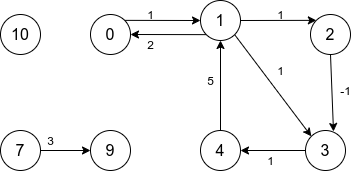
\includegraphics[keepaspectratio,width=0.5\textwidth]{img/03-graphs/data_struct_gr.png}
            \end{center}
            \caption{An example graph used throughout this section.} 
            \label{data_struct-ex}
        \end{figure}
        
        \subsection*{Unordered Edge List}
            The simplest representation uses an unordered list of edges. 
            That is each element of the data structure carries the information of exactly one edge. 
            For example in a directed, weighted graph, the indices of the source and target node and the weight of the edge are one entry. 
            Additionally, an edge list needs to store a list of vertex indices, to represent nodes with no edges.
            Overall this results in $\mathcal{O}|E| + |V|$ space complexity.
            
            The number of nodes can be retrieved in $\mathcal{O}(1)$ assuming that the list data structure stores its size as a field. 
            The same is true for edges.
            Finding a vertex requires inspecting the list of vertices, thus $\mathcal{O}(|V|)$. 
            Assuming the list stores a pointer to its tail, vertex insertion's asymptotic runtime is $\mathcal{O}(1)$. 
            Deleting a vertex requires a pass over all edges to remove the ones including the particular vertex, in total $\mathcal{O}(|E|)$.
            For edges, the basic operations find, and remove can be executed in linear runtime, i.e. $\mathcal{O}(|E|)$.
            Edge insertion's asymptotic runtime is $\mathcal{O}(1)$, again assuming the list stores a reference to its tail. 
            Deciding whether two vertices are adjacent requires iterating over the list of edges, that is 
            $\mathcal{O}(|E|)$ runtime.
            Finally, finding the neighborhood $N_v$ of a vertex requires again a scan of all edges, i.e. an asymptotic runtime of $\mathcal{O}(|E|)$. 
            The same is true for the incoming and outgoing sets of a vertex.
            An example of this data structure is shown in Listing~\ref{edgelist}.
            
            \begin{figure}[htp]
            \begin{center}
            \begin{minipage}{0.5\textwidth}
            \begin{minted}[fontsize=\footnotesize]{bash}
            0 1 2 3 4 7 9 10
            \end{minted}
            \begin{minted}{bash}
            0 1 1
            1 0 2
            1 2 1
            2 3 -1
            1 3 1
            3 4 1
            4 1 5
            7 9 3
            \end{minted}
            \end{minipage}%
            \hfill%
            \begin{minipage}{0.5\textwidth}
            \begin{minted}[fontsize=\footnotesize]{bash}
            0 1 1
            1 0 2
            1 2 1
            2 3 -1
            1 3 1
            3 4 1
            4 1 5
            5 6 3
            \end{minted}
            \end{minipage}
            \end{center}
            \caption{%
                An example of the edge list representation of a graph.%
                The left-hand side uses a list to encode vertex indices, while the right-hand side assumes consecutive indexes.%
            }
            \label{edgelist}
            \end{figure}

        \subsection*{Adjacency Matrix}
            An adjacency matrix of a graph $G$ is a $|V|\times|V|$ matrix where a non-zero entry corresponds to an edge with the weight being the value of that entry. 
            Let $A \in |V|\times|V|, \ u, v \in \{0, \dots, |V| - 1\}$ and $w_{u,v}$ the weight of the edge $e = (u,v) \in E$ then
            \[ a_{uv} = \begin{cases}
                        w_{u,v} & \text{if } (u,v) \in E \\
                        0 & \text{otherwise}
                        \end{cases}
            \]
            Additionally, to model non-consecutive indices, one needs to store a mapping from the actual vertex index to the one used in the matrix --- usually represented by a 2D array. 
            It is also important to note, that adjacency matrix representations are not able to represent multi-graphs without further modification.
            The space complexity of an adjacency matrix is thus $\mathcal{O}(|V|^2 + |V|)$.
                    
            The number of nodes can be retrieved in $\mathcal{O}(1)$, as it's simply the size of the mapping that is stored.
            For the number of edges, one needs to iterate over all elements of the matrix and count the non-zero entries, which requires one to touch $\mathcal{O}(|V|^2)$ elements.
            Finding a vertex is just an array lookup, thus $\mathcal{O}(1)$.
            Insertion requires adding one row and one column to the matrix, as well as one entry to the mapping. 
            This includes reallocating the matrix which is non-deterministic and independent of the matrix size. But it also requires copying all elements to the new matrix, such that we can estimate the overall asymptotic runtime of $\mathcal{O}(|V|^2)$.
            Deleting a vertex is similar. Either one leaves a gap that may be used on subsequent insertions and simply marks the true id in the mapping as deleted, which would be an $\mathcal{O}(1)$ operation. 
            Alternatively one could immediately reallocate the matrix to free the extra row and column as well as the extra field in the mapping. 
            This would again be non-deterministic, but can again be estimated by copying the elements from the former matrix $\mathcal{O}(|V-1|^2) = \mathcal{O}(|V|^2)$.
            For edges, the basic operations find, insert and remove can be executed in constant runtime, i.e. $\mathcal{O}(1)$, as simple array access.
            Deciding whether two vertices are adjacent requires just reading what is in the particular array at the index of the two nodes, that is $\mathcal{O}(1)$ runtime.
            Finally, finding the neighborhood $N_v$ of a vertex requires again a scan of a row and a column i.e. an asymptotic runtime of $\mathcal{O}(2|V|)$. For the incoming and outgoing sets of a vertex, one needs to access only either a row or a column resulting in $\mathcal{O}(|V|)$ steps per operation.
            An example of this data structure is shown in Listing~\ref{adm}.
            
            \begin{figure}[htp]
            \begin{center}
            \begin{minted}[fontsize=\footnotesize]{bash}
                0 1 2 3 4 5 6 7
                0 1 2 3 4 7 9 10
            \end{minted}
            \begin{minted}{bash}
                0 1 0  0 0 0 0 0
                2 0 1  1 0 0 0 0
                0 0 0 -1 0 0 0 0
                0 0 0  0 1 0 0 0
                0 5 0  0 0 0 0 0
                0 0 0  0 0 0 3 0
                0 0 0  0 0 0 0 0
                0 0 0  0 0 0 0 0
            \end{minted}
            \end{center}
            \caption{An example of the adjacency matrix representation of a graph.}
            \label{adm}
            \end{figure}
        
        \subsection*{Incidence Matrix}
            An incidence matrix of a graph $G$ is an $|V| \times |E|$ matrix, where each column corresponds to an edge. 
            Each entry in a column is either the positive weight, if the node is the target of the edge, or the negative weight if the node is the source of the edge. Self-loops require a slight extension of this syntax because here one node would be both source and target such that the entry is zero. One option is to just put the weight as an entry of the node.  Another problem is that incidence matrices can not represent negative weights without further extensions.        
            Let $u,v \in \{0, |V|-1\}, j \in \{0, |E|-1\}, A \in |V| \times |E|$ and $a_{v,j}$ the entry at row $v$ and column $j$ of $A$. Let further $w_j$ be the weight of the edge $e_j = (u,v) \in E$. Then 
            \[         a_{vj} = \begin{cases}
                        -w_{v,u} & \text{if } e_j = (v,u) \in E \\
                        w_{u,v} & \text{if } e_j = (u,v) \in E \\
                        0 & \text{otherwise}
                        \end{cases}
            \]
            
            As with adjacency matrices, to be able to represent non-consecutive indices, we need to store a mapping from the true node indices to the ones used in the matrix.
            The space requirements are thus $\mathcal{O}(|V| \cdot |E| + |V|) = \mathcal{O}(|V| \cdot |E|)$.
            
            The number of nodes can be retrieved in $\mathcal{O}(1)$, as it's simply the size of the mapping that is stored.
            The number of edges can also be retrieved in $\mathcal{O}(1)$ as it's the second dimension of the matrix.
            Finding a vertex is just an array lookup, thus $\mathcal{O}(1)$.
            Insertion requires adding one row and one column to the matrix, as well as one entry to the mapping, as with adjacency lists. 
            Thus the complexity is again the cost of copying the whole matrix $\mathcal{O}(|V| \cdot |E|)$. 
            The same is true for deleting a vertex.         
            To find an edge, one needs to scan one row of either the source or the target node of the edge, which requires $\mathcal{O}(|E|)$ steps.
            Insertion and removal of edges correspond to the case of vertices.
            One would need to reallocate the matrix and copy all elements resulting in an asymptotic runtime complexity of $\mathcal{O}(|V| \cdot |E|)$. 
            Deciding whether two vertices are adjacent requires reading one row and checking for each non-zero element, if the entry in the other nodes row is also non-zero, which has $\mathcal{O}(|E|)$ runtime.        
            Finally, finding the neighborhood $N_v$ of a vertex requires again a scan of a row and checking all non-zero entry columns for the neighbor i.e. an asymptotic runtime of $\mathcal{O}(|E|)$. 
            For the incoming and outgoing sets, the procedure is almost the same. 
            The difference is, that only positive or negative non-zero columns --- depending on whether the incoming or outgoing neighbors shall be returned -- have to be checked.
            An example of this data structure is shown in Listing~\ref{incm}.
        
        \begin{figure}[htp]
         \begin{center}
         \begin{minted}[fontsize=\footnotesize]{bash}
            0 1 2 3 4 5 6 7
            0 1 2 3 4 7 9 10
          \end{minted}
          \begin{minted}{bash}
            -1  2  0  0    0   0  0
            1  -2 -1 -(-1) 0   5  0
            0   0  1  0    0   0  0
            0   0  0  (-1) 1   0  0
            0   0  0  0    1  -5  0
            0   0  0  0    0   0  0
            0   0  0  0    0   0 -3
            0   0  0  0    0   0  3
          \end{minted}
         \end{center}
         \caption{An example of the incidence matrix representation of a graph.}
         \label{incm}
        \end{figure}
        
        \subsection*{Adjacency List}
        In an adjacency list, there is an entry for each vertex in the graph. 
        Each such entry stores the nodes that are adjacent to the vertex, i.e. its neighborhood $N_v$. 
        It is important to note, that in most implementations only $N_v |_\text{out}$ is the content of the adjacency list.
        When we sum $|N_v |_\text{out}|$ over all vertices of the graph, we count each edge once.
        The space complexity here is $\mathcal{O}(|V| + |V| \cdot \text{deg}(V)) = \mathcal{O}(|V| + |E|)$, as we store each node once and then for each relationship one more node in the corresponding adjacency list containing $N_v |_\text{out}$.

        The number of nodes can be retrieved in $\mathcal{O}(1)$, as it's the size of the list.
        For retrieving the number of edges, one needs to iterate over all elements of the node list and sum over their respective adjacency list. 
        This requires $\mathcal{O}(|V| \cdot \text{deg}(V)) = \mathcal{O}(|E|)$ operations.
        Finding a vertex is just a lookup, thus in $\mathcal{O}(1)$.
        Inserting a vertex means simply appending an element to a list which is in $\mathcal{O}(1)$.
        Deleting a vertex requires iterating over all nodes and their adjacency list in order to remove the occurrences as adjacent node and is in $\mathcal{O}(|V| \cdot \text{deg}(V)) = \mathcal{O}(|E|)$.
        Finding an edge can be done by checking the adjacency list of the source node, and requires looking at $\mathcal{O}(\text{deg}(V))$ elements.
        For the insertion of an edge, one needs to append one element to the end of the adjacency list of the source node, which can be done in $\mathcal{O}(1)$.
        Removing an edge again requires iterating over the adjacency list of the source node and remove the corresponding entry which is again in $\mathcal{O}(\text{deg}(V))$.        
        Deciding whether two vertices are adjacent can be checked by looking at the adjacency lists of two nodes, that is $\mathcal{O}(2 \cdot \text{deg}(V)) = \mathcal{O}(\text{deg}(V))$ runtime.        
        Finally, the outgoing neighborhood of a vertex is already stored and can be returned in $\mathcal{O}(1)$.
        In contrast for the incoming neighborhood one needs to access all vertices' adjacency list and see if the particular vertex is contained in it, resulting in $\mathcal{O}(|V| \cdot \text{deg}(V)) = \mathcal{O}(|E|)$ operations.
        Finding the neighborhood $N_v$ of a vertex requires to do both of the above queries, that is $\mathcal{O}(|V| \cdot \text{deg}(V) + 1) = \mathcal{O}(|V| \cdot \text{deg}(V))  = \mathcal{O}(|E|)$ operations.  
        Note that in undirected graphs, both directions of all edges exist, i.e. $N_v = N_v |_\text{out} = N_v |_\text{in}$. This means for undirected graphs all neighborhood queries are in $\mathcal{O}(1)$.      
        An example of this data structure is shown in Listing~\ref{adjl}.
        
        \begin{figure}[htp]
         \begin{center}
          \begin{minted}[fontsize=\footnotesize]{bash}
            0 -> (1, 1)
            1 -> (0, 2) -> (2,1) -> (3, 1)
            2 -> (3, -1)
            3 -> (4, 1)
            4 -> (1, 5)
            7 -> (9, 3)
            9
            10
          \end{minted}
         \end{center}
         \caption{An example of the adjacency list representation of a graph.}
         \label{adjl}
        \end{figure}
        
        \subsection*{Incidence List}\label{inci}
            This representation is also called incidence table in \autocite{Gross1998GraphTA}.
            The incidence list of a graph $G$ stores for each vertex $v \in V$ the list of edges it is connected to. 
            The space requirements are thus $\mathcal{O}(|V| + |V| \cdot \text{deg}(V) + |E|) = \mathcal{O}(|V| + |E|)$. 
            In contrast to adjacency lists, incidence lists do not only store the connected vertices but the edges. 
            This comes with an additional cost of $|E|$ memory but is beneficial when it comes to accessing information. 
            Another benefit is that the additional costs can be mitigated by using references.
            
            Most of the operations have the same complexity class as when using adjacency lists and the same operations are needed. 
            Differences occur first when removing a vertex
            Instead of having to iterate over all lists and check if the vertex is contained, it is sufficient to look the relevant lists up in the vertexes' list and delete them resulting in $\mathcal{O}(\text{deg}(V))$ operations.        
            Differences also occur, when accessing the neighborhood. 
            As all edges that are incident to a node are stored, finding all neighbors is an $\mathcal{O}(1)$ operation. 
            Considering the incoming and outgoing neighborhoods, one only needs to filter the list of incident edges accordingly, which has length $\mathcal{O}(\text{deg}(V))$.
            An example of this data structure is shown in Listing~\ref{incidencel}.
        
            \begin{figure}[htp]
            \begin{center}
            \begin{minted}[fontsize=\footnotesize]{bash}
                0 -> (0, 1, 1) -> (1, 0, 2)
                1 -> (1, 0, 2) -> (1, 2, 1) -> (1, 3, 1) -> (4, 1, 5) -> (0, 1, 1)
                2 -> (2, 3, -1) -> (1, 2, 1)
                3 -> (3, 4, 1) -> (1, 3, 1) -> (2, 3, -1)
                4 -> (4, 1, 5)
                7 -> (7, 9, 3)
                9 -> (7, 9, 3)
                10
            \end{minted}
            \end{center}
            \caption{An example of the incidence list representation of a graph.}
            \label{incidencel}
            \end{figure}
            
        
        
        \subsection*{Summary}
            While edge lists can represent all variations of graphs, the asymptotic runtime for many operations is linear in the number of edges. 
            These are unacceptable costs in many cases.
            
            An adjacency matrix improves the performance for lookups and updates and is thus the standard data structure for many computation-heavy tasks and widely used by libraries as Eigen, openBLAS, and the Intel math kernel library (MKL)~\autocite{MatrixStorageSchemes-2021-03-05, EigenTheMatrixclass-2020-12-05, MatrixStorageSchemes-1999-10-01}. 
            When dealing with multi-graphs, the adjacency matrix representation requires additional arrays (one per edge ``type``) or is not able to canonically represent them.       
            The incidence matrix is not able to represent self-loops and negative weights without modification but has some interesting relationships with other matrices. 
            For example, if one multiplies the incidence matrix with its transpose, one gets the sum of the adjacency matrix and the gradient matrix, i.e. the laplacian matrix~\autocite{brouwer2011spectra}. 
            Furthermore, it's useful in physical flow problems and simulations, e.g. when computing the current and resistances in a graph or when simulating micro-circuits~\autocite{weinberg1958kirchhoff}.
            Even though the incidence matrix requires less space, both options are rather unfeasible when storing large graphs and the incidence matrix provides even worse access times than edge lists.        
            As a side note, The compressed sparse row and compressed sparse column storage formats are very similar to adjacency lists. 
            Instead of using lists, three arrays are used. 
            The first one maps the node to the start index of its relationship in the other two arrays. 
            The other two arrays store the adjacent nodes and the weight of the relationship respectively. 
            CSR/CSC and adjacency lists share most of the algorithmic traits while requiring the least storage. 
            These formats are used for sparse matrix arithmetics in some of the most popular matrix arithmetics libraries, like~\autocite{MatrixStorageSchemes-2021-03-05, EigenTheMatrixclass-2020-12-05, MatrixStorageSchemes-1999-10-01}. 
            
            Finally, the adjacency and incidence lists are quite similar in many aspects. Both require linear storage space --- which is optimal without further compression. 
            Even though not optimal for the operations \mintinline{c}{get}, \mintinline{c}{insert} and \mintinline{c}{remove}, both data structures provide access times that are asymptotically better than linear in most cases.
            If the edges are distributed uniformly, we have an upper bound for the average degree of $\text{deg}(V) = \frac{2|E|}{|V|} \leq \frac{2 |V|^2}{|V|} = 2 |V|$.
            In real networks, the distribution is often non-uniform but can be modeled using e.g. binomial, Poisson, or power-law type~\autocite{holme2019rare}. 
            A power law distribution would mean that there exist few nodes with a high degree and a lot of nodes with a rather low degree. 
            What is also very appealing is the fact that the adjacency list and especially the incidence list enables one to return the neighborhood of a vertex in a constant or degree-based amount of time. 
            When it comes to traversals of a graph, these are crucial operations as we will see in the next subsection. 
            
            In Table \ref{sumtabds} we summarize the space and runtime complexities of the described data structures and the operations that act upon them. 
            
            \begin{table}
            \begin{center}
                \begin{tabular}[c]{l l l l l l} \toprule
                \multirow{2}{*}{} & Edge List & Adjacency & Incidence & Adjacency  & Incidence \\ 
                & &  Matrix & Matrix & List & List \\ \midrule
                Space & $\mathcal{O}(|V| + |E|)$ & $\mathcal{O}(|V|^2)$ & $\mathcal{O}(|V| \cdot |E|)$ & $\mathcal{O}(|V| + |E|)$ & $\mathcal{O}(|V| + |E|)$ \\
                \mintinline{c}{size} $|E|$ & $\mathcal{O}(1)$ & $\mathcal{O}(|V|^2)$ & $\mathcal{O}(1)$ & $\mathcal{O}(|E|)$ & $\mathcal{O}(|E|)$ \\
                \mintinline{c}{find} $v$ & $\mathcal{O}(|V|)$ & $\mathcal{O}(1)$ & $\mathcal{O}(1)$ & $\mathcal{O}(1)$ & $\mathcal{O}(1)$ \\
                \mintinline{c}{insert} $v$ & $\mathcal{O}(1)$ & $\mathcal{O}(|V|^2)$ & $\mathcal{O}(|V| \cdot |E|)$ & $\mathcal{O}(1)$ & $\mathcal{O}(1)$ \\
                \mintinline{c}{remove} $v$ & $\mathcal{O}(|E|)$ & $\mathcal{O}(|V|^2)$ & $\mathcal{O}(|V| \cdot |E|)$ & $\mathcal{O}(|E|)$ & $\mathcal{O}(\text{deg}(V))$ \\
                \mintinline{c}{find} $e$ & $\mathcal{O}(|E|)$ & $\mathcal{O}(1)$ & $\mathcal{O}(|E|)$ & $\mathcal{O}(\text{deg}(V))$ & $\mathcal{O}(\text{deg}(V))$ \\
                \mintinline{c}{insert} $e$ & $\mathcal{O}(1)$ & $\mathcal{O}(1)$ & $\mathcal{O}(|V| \cdot |E|)$ & $\mathcal{O}(1)$ & $\mathcal{O}(1)$ \\
                \mintinline{c}{remove} $e$ & $\mathcal{O}(|E|)$ & $\mathcal{O}(1)$ & $\mathcal{O}(|V| \cdot |E|)$ & $\mathcal{O}(\text{deg}(V))$ & $\mathcal{O}(\text{deg}(V))$ \\
                \mintinline{c}{is_adjacent} $u, v$ & $\mathcal{O}(|E|)$ & $\mathcal{O}(1)$ & $\mathcal{O}(|E|)$ & $\mathcal{O}(\text{deg}(V))$ & $\mathcal{O}(\text{deg}(V))$ \\
                \mintinline{c}{get} $N_v$ & $\mathcal{O}(|E|)$ & $\mathcal{O}(|V|)$ & $\mathcal{O}(|E|)$ & $\mathcal{O}(|E|)$ & $\mathcal{O}(1)$ \\
                \mintinline{c}{get} $\text{In}_v$ & $\mathcal{O}(|E|)$ & $\mathcal{O}(|V|)$ & $\mathcal{O}(|E|)$ & $\mathcal{O}(|E|)$ & $\mathcal{O}(\text{deg}(V))$ \\
                \mintinline{c}{get} $\text{Out}_v$ & $\mathcal{O}(|E|)$ & $\mathcal{O}(|V|)$ & $\mathcal{O}(|E|)$ & $\mathcal{O}(1)$ & $\mathcal{O}(\text{deg}(V))$ \\ \bottomrule
            \end{tabular}
            \end{center}
            \caption{Space and runtime complexity comparison of the different data types.}
            \label{sumtabds}
            \end{table}

    \newpage
    \section{Algorithms}\label{queries}
        There are many kinds of graph problems and algorithms tackling them. As we are interested in the access patterns of traversal-based queries we are going to focus on traversal and shortest path algorithms. We also look at some partitioning methods as these are used quite frequently when addressing the issues in the next chapter.
        Nevertheless, other classes of algorithms are of equal importance and have many use cases, like flow problems, finding graph isomorphisms, identifying minimal spanning trees, determining the centrality of a node, and others.
        Comprehensive resources for these problems can be found in~\autocite{steger2007diskrete, Gross1998GraphTA, aho1974design, cormen2009introduction, Goodrich2014AlgorithmDA}.
        
        \subsection{Traversal Algorithms}
            Visiting the nodes in a graph is known as graph traversal. 
            The order in which the nodes are visited is given by the respective algorithm. 
            The two most important graph traversal schemas are the breadth-first search and the depth-first search. 
            Another such schema is the random walk, which is not quite a traversal but rather generates an arbitrary walk. 
            However, it defines, in which order nodes are visited even if it does not guarantee that all nodes are visited and that all nodes are visited exactly once.
            \subsubsection*{Depth-First Search}
                One description of the depth-first search (DFS) was authored by Charles-Pierre Trémaux in 1818.
                Even though the work was published a lot later, this is the first appearance in modern citation history~\autocite{lucas1891recreations}. 
                He used so-called Trémaux trees to solve arbitrary mazes. 
                Each result of a depth-first search is such a Trémaux tree.
                These have the property that every two adjacent vertexes are in an ancestor-descendant relationship.
                Even though Trémaux trees themselves are interesting --- for example, all Hamiltonian paths are Trémaux trees --- we focus on the description of the depth-first search.        
                Depth-first search is very similar to backtracking. Chase one path until it proves to be a dead end. 
                Go back to the point where you can take a different path, chose that path to chase and repeat. 
                In fact, Donald Knuth considers depth-first search and backtracking to be the same algorithm, as both are acting upon a graph. 
                However, when backtracking is used, the graph is often implicit~\autocite{Knuth2000DancingL}.        
                Even though DFS is a general traversal schema -- go deep first -- it can also be used for other purposes like finding shortest paths, connected components, testing planarity, and many more. 
                        
                \begin{algorithm}[htp]
                    \KwIn{Graph $G = (V,E)$, start vertex id v\_id, direction $d$}
                    \KwOut{Search numbers DFS, predecessor edges parent}
                    \hrulealg
                    \Begin{
                        dfs $\leftarrow$ array initialized to $-1$\;
                        parents $\leftarrow$ array initialized to $-1$\;
                        node\_stack $\leftarrow$ create\_stack()\;
                        
                        push(node\_stack, v\_id)\;
                        
                        \While{node\_stack non-empty}{
                            node\_id $\leftarrow$ pop(node\_stack)\;
                            current\_node\_edges $\leftarrow$ expand($G$, v\_id, $d$)\;
                            
                            \For{edge $\in$ current\_node\_egdes}{
                                \If{dfs[edge.other\_v\_id] $= -1$}{
                                    dfs[edge.other\_v\_id] $\leftarrow$ dfs[node\_id] + 1\;
                                    push(node\_stack, edge.other\_v\_id)\;
                                    parent[edge.other\_id] $\leftarrow$ edge.id\;
                                }
                            }
                        }
                        \Return distances, parents\;
                    }
                \caption{Pseudo-code for a depth-first search on a graph $G$.}\label{dfs}
                \end{algorithm}
                A pseudo-code description of it is given in Algorithm~\ref{dfs}. 
                This version continues its search at the last found edge instead of the last visited edge. 
                This is to enable the usage of the implementation for other problems like finding spanning trees, cycles, or paths.
                The runtime is again dependent on the data structure, that is used and again the runtime for querying the neighborhood of a node is the varying term. 
                Each node is visited exactly once and by the handshaking lemma~\autocite{Gross1998GraphTA} it should be clear that we visit each edge twice resulting in an overall worst-case runtime of $\mathcal{O}(|V|+|E|)$. 
                Regarding space complexity, the worst-case is that the node stack contains all nodes, i.e. that it is traversed without repetitions or --- put differently --- backtracking. 
                The result is a worst-case space complexity of $\mathcal{O}(|V|)$.
            
            \subsubsection*{Breadth-First Search} 
                The first description of breadth-first search (BFS) in modern science was given by Konrad Zuse in the course of his Ph.D. thesis on the ''Plankalkühl``. 
                He used it to find connected components~\autocite{zuse1948allgemeinen}. 
                The schema of the breadth-first search was also used to find shortest path solutions for mazes and to wire up placed electrical components on a printed circuit board (PCB).
                The general traversal scheme in breadth-first search is to explore all next neighbors before continuing with those who are more steps away. 
                Thus it first explores one ''level`` exhaustively, before continuing to the next one. 
                In other words, the only difference between DFS and DFS is the data structure that is used. While DFS uses a stack and thus always inspects the element that was inserted last, BFS uses a queue.
                That means it inspects the element that was inserted first.
                Illustrative comparison of DFS and BFS is shown in Figure~\ref{dfs-bfs}. 
                
                \begin{figure}[htp]
                \begin{center}
                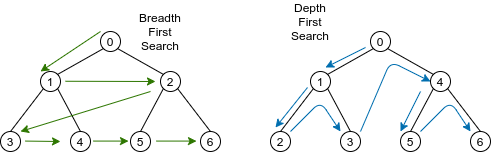
\includegraphics[keepaspectratio,width=0.7\textwidth, height=0.3\textheight]{img/03-graphs/bfs-dfs.png}
                \end{center}
                \caption{Comparison between a DFS and a BFS traversal.}\label{dfs-bfs}
                \end{figure}
                
                Like the DFS, the BFS traversal schema can be used to find shortest paths, maximum flows and to test if a graph is bipartite. 
                Space and runtime complexity of the BFS is similar to the complexities of DFS. $\mathcal{O}(|V|)$ space, when all nodes are stored in the queue at the same time. 
                $\mathcal{O}(|V| + |E|)$ since all vertices are visited and each edge is visited twice by the handshake lemma. 
                Pseudo-code for the BFS traversal-scheme is shown in Algorithm~\ref{bfs}. 
                We again make the assumption, that we are using an incidence list as s data structure and that the expand operator is implemented accordingly.

                \begin{algorithm}[htp]
                    \KwIn{Graph $G = (V,E)$, start vertex id v\_id, direction $d$}
                    \KwOut{Search numbers bfs, predecessor edges parent}
                    \hrulealg
                    \Begin{
                        bfs $\leftarrow$ array initialized to $-1$\;
                        parents $\leftarrow$ array initialized to $-1$\;
                        node\_queue $\leftarrow$ create\_queue()\;
                        
                        enqueue(node\_queue, v\_id)\;
                        
                        \While{node\_queue non-empty}{
                            node\_id $\leftarrow$ dequeue(node\_queue)\;
                            current\_node\_edges $\leftarrow$ expand($G$, v\_id, $d$)\;
                            
                            \For{edge $\in$ current\_node\_egdes}{
                                \If{bfs[edge.other\_v\_id] $= -1$}{
                                    bfs[edge.other\_v\_id] $\leftarrow$ bfs[node\_id] + 1\;
                                    enqueue(node\_queue, edge.other\_v\_id)\;
                                    parent[edge.other\_id] $\leftarrow$ edge.id\;
                                }
                            }
                        }
                        \Return distances, parents\;
                    }
                \caption{Pseudo-code for a breadth-first search on a graph $G$.}\label{bfs}
                \end{algorithm}
                
            \subsubsection*{Random Walk}\label{rand-w}
                A random walk is a stochastic process, originally defined by Karl Pearson posing the following problem to the readers or the journal nature in 1905~\autocite{pearson1905problem}: 
                \begin{quote}
                    A man starts from a point $O$ and walks $I$ yards in a straight line; he then turns through any angle whatever and walks another $I$ yards in a second straight line. 
                    He repeats this process n times. 
                    I require the probability that after these $n$ stretches he is at a distance between $r$ and $r + \delta r$ from his starting point, $O$.
                \end{quote}
                The problem has gathered wide interests and has many connections ranging from financial mathematics~\autocite{bachelier1900theorie}, over physics and biology (Brownian motion\autocite{brown1828xxvii}) to pure mathematics~\autocite{wiener1976collected}. 
                Random walks are modeled mathematically using Markov chains.            
                The purely mathematical theory is outlined in a comprehensive survey~\autocite{lovasz1993random}. 
                Our focus will remain database-oriented, and traversal-based.
                In~\autocite{fouss2007random} the authors show, that the generated random walks can be used to compute the similarities of nodes in a graph. 
                This insight is used by a method described in the next chapter.
                
                \begin{algorithm}[htp]
                    \KwIn{Graph $G = (V,E)$, number of steps $n$, start vertex id $v\_id$, direction $d$}
                    \KwOut{A walk $(e_0, \dots, e_{n-1})$}
                    \hrulealg
                    \Begin{
                        visited\_edges $\leftarrow$ edge\_t[$n$]\;
                        current\_node\_edges $\leftarrow$ expand($G$, $v\_id$, $d$)\;
                        
                        \For{$i$ from $0$ to $n - 1$}{
                            edge $\leftarrow$ current\_node\_edges[random() $\%$ size(current\_node\_edges)]\;
                            append(visited\_edges, edge)\;
                            current\_node\_edges $\leftarrow$ expand($G$, edge.other\_v\_id, $d$)\;
                        }
                        \Return visited\_edges\;
                    }
                \caption{Pseudo-code for a random walk on a graph $G$.}\label{random_walk}
                \end{algorithm}
                
                Pseudo-code describing the algorithm can be found in Algorithm~\ref{random_walk}. 
                The code makes two assumptions. The function \mintinline{c}{random()} returns an unsigned integer by drawing from a uniform distribution. 
                The function \mintinline{c}{expand} returns the edges with a certain direction of a vertex, given a graph, a vertex (id), and the respective direction.
                
                The runtime complexity of a random walk can be estimated using the number of steps and the average degree of each node in the graph. 
                In each of the $n$ steps, we have to construct the list of edges of the currently considered vertex, which has a length of $\mathcal{O}(\text{deg}(V))$. 
                How fast this construction depends on the data structure that is used. 
                The overall average runtime complexity is $\mathcal{O}(n \cdot \text{deg}(V))$ for incidence lists. 
                For the other data structures, one has to replace the $\text{deg}(V)$ term with the respective runtime of retrieving the neighborhood of vertex. 
                The average space complexity of a random walk is $\mathcal{O}(\text{deg}(V))$.
        
    \subsection{Shortest Path Algorithms}
        The shortest path problem is defined by finding the shortest path between nodes efficiently.
        The algorithms below tackle two specific subproblems:
        \begin{enumerate}
         \item the Dijkstra algorithm finds shortest paths between a single source node and all other nodes in the graph.
         \item the A$^*$ algorithm finds the shortest path between a single source and a single target node.
        \end{enumerate}
        The difference in the problem setting allows for certain heuristic optimizations. 
        While Dijkstra's algorithm is slower, it returns more information.
        The A$^*$ algorithm's narrower focus allows it to inspect fewer elements based on a heuristic and is bound by Dijkstra's algorithm in the worst-case.

        \subsubsection*{Dijkstra} 
            In the original formulation, Edsger Dijkstra formulated the algorithm as a solution to the problem of finding the shortest paths between two nodes~\autocite{dijkstra1959note}. 
            Many variants and extensions exist of which we are going to discuss two --- A$^*$ and ALT~\autocite{hart1968formal, goldberg2005computing}. 
            One slight variation makes it possible to find all the shortest paths from a given source node.
            The algorithm however restricts on the graph.
            Only positive weights are allowed as otherwise, a negative cycle results in an infinite loop~\autocite{cormen2009introduction}. 
            
            Conceptually Dijkstra's algorithm assigns each node in the graph a distance. 
            The source vertex has the distance 0, while all other vertices have a distance of infinity at the beginning.
            Then it gradually considers the next ''shortest`` edge to take.
            That is the distance of the already taken path to a certain node (at the beginning it's zero) is added to an edge weight such that the sum of both is minimal. 
            To efficiently compute the minimum a binary heap-based priority queue or a Fibonacci heap is used to define the traversal order. 
            An array stores the distances from the source to the already visited nodes, while the queue is filled with their neighbors along with the distance to them (i.e. the path to the predecessor plus the weight of the edge to be taken). 
            The vertex with the shortest total distance is visited until all vertices are visited or the target vertex is reached.
            
            Pseudo-code for the variant that computes all shortest paths can be found in Algorithm~\ref{dijkstra}. 
            The runtime complexity of Dijkstra's algorithm is $\mathcal{O}(|E| \cdot T_d + |V| \cdot T_m)$ where $T_d, T_m$ stand for the complexities to update the distance of a path and to extract the minimum.
            Besides the new necessity to select the element to inspect based on priorities and to maintain those, the runtime complexity is equivalent to what we had with BFS.        
            Using a binary heap-based priority queue yields sub-optimal runtime:
            $T_d, T_m \in \mathcal{\log(|V|)}$. 
            Overall the asymptotic runtime complexity using a min-priority queue is $\mathcal{O}((|V| + |E|)\log(|V|))$~\autocite{Goodrich2014AlgorithmDA}.        
            One can also use plain arrays, which requires a minimum search and no update of the priority. 
            The minimum search is linear, i.e. $\mathcal{O}(|V|)$ and priorities can be updated in $\mathcal{O}(1)$. 
            Overall we have $\mathcal{O}(|E| + |V|^2)$~\autocite{Goodrich2014AlgorithmDA}.        
            Finally, more advanced data structures can be used, like a Fibonacci-Heap~\autocite{cormen2009introduction}. 
            These make it possible to update the priority in $\mathcal{O}(1)$ and still find the minimum in $\mathcal{\log(|V|)}$. 
            This yields the optimal asymptotical runtime of $\mathcal{O}(|E| + |V|\log(|V|))$. 
            The worst-case space complexity is again $\mathcal{O}(|V|)$, that is when all nodes are stored in the queue at the same time. 
            As there is only one shortest path (paths of equal size are discarded) to each node, the queue contains each node only once.
            
            \begin{algorithm}[htp]
                \KwIn{Graph $G = (V,E)$, source vertex id v\_id, direction $d$}
                \KwOut{Path distance distances, predecessor edges parent}
                \hrulealg
                \Begin{
                    distances $\leftarrow$ array initialized to $\infty$\;
                    parents $\leftarrow$ array initialized to $-1$\;
                    path\_queue $\leftarrow$ create\_min\_prio\_queue()\;
                    
                    enqueue(path\_queue, v\_id)\;
                    
                    \While{path\_queue non-empty}{
                        node\_id $\leftarrow$ dequeue(path\_queue)\;
                        current\_node\_edges $\leftarrow$ expand($G$, v\_id, $d$)\;
                        
                        \For{edge $\in$ current\_node\_egdes}{
                            \If{distances[edge.other\_v\_id] $\geq$ distances[node\_id] + edge.weight}{
                                distances[edge.other\_v\_id] $\leftarrow$ distances[node\_id] + edge.weight\;
                                enqueue(path\_queue, edge.other\_v\_id)\;
                                parent[edge.other\_id] $\leftarrow$ edge.id\;
                            }
                        }
                    }
                    \Return distances, parents\;
                }
            \caption{Pseudo-code of the Dijkstra's algorithm for finding shortest paths from a node $v$ to all other nodes in a graph $G$.}\label{dijkstra}
            \end{algorithm}
        
        
        \subsubsection*{A*}
            The A$^*$ was originally invented in the late 60's to be used for path planning of a robot. 
            It's an extension of Dijkstra's algorithm, that does not just use the distance as metric of priority, but adds a heuristic $h: V \rightarrow \mathbb{R}$ to the distance.
            $v \in V: f(v) = \text{distance}(v) + h(v)$, that has to fulfill certain conditions.
            With $u,v \in V$ and $\min\text{ distance}(u)$ the minimal distance from the  vertex $u$ to the goal vertex
            \[ \forall u,v: h(u) \leq d(u, v) + h(v) \wedge h(u) \leq \min\text{ distance}(u).
            \]
            The former condition is called consistency, the latter admissibility. 
            As all consistent heuristics are admissible the first condition is sufficient.
            An example for graphs using the Euclidean coordinate system is the Euclidean distance~\autocite{hart1968formal}.
            
            Algorithm~\ref{a-star} shows pseudo-code for the algorithm. The runtime is of course dependent on the complexity of the heuristics.
            Overall we have the same worst-case complexity as with Dijkstra's algorithm for the constant heuristic
            $\forall v \in V: h(v) = 0$. 
            The best-case of the A$^*$ algorithm is when the heuristic is equal to the distance from the current vertex to the goal vertex. 
            Then exactly $\min \text{distance}$ nodes are visited and the algorithm is in $\mathcal{O})\min \text{distance})$, which is the global optimum for a single source shortest path problem.
            
            \begin{algorithm}[htp]
                \KwIn{Graph $G = (V,E)$, heuristic $h$, source vertex id v\_source, target node v\_target, direction $d$}
                \KwOut{Path p}
                \hrulealg
                \Begin{
                    parents $\leftarrow$ array initialized to $-1$\;
                    path\_queue $\leftarrow$ create\_min\_prio\_queue()\;
                    
                    enqueue(path\_queue, v\_id)\;
                    
                    \While{path\_queue non-empty}{
                        node\_id $\leftarrow$ dequeue(path\_queue)\;
                        
                        \If{node\_id = v\_target}{
                            \Return construct\_path(parents)\;
                        }
                        
                        current\_node\_edges $\leftarrow$ expand($G$, v\_id, $d$)\;
                        
                        \For{edge $\in$ current\_node\_egdes}{
                            \If{distances[edge.other\_v\_id] $\geq$ distances[node\_id] + edge.weight + $h($edge.other\_v\_id)}{
                                distances[edge.other\_v\_id] $\leftarrow$ distances[node\_id] + edge.weight + $h($edge.other\_v\_id$)$\;
                                enqueue(path\_queue, edge.other\_v\_id)\;
                                parent[edge.other\_id] $\leftarrow$ edge.id\;
                            }
                        }
                    }
                    \Return empty\_path()\;
                }
            \caption{Pseudo-code of the A$^*$ algorithm for finding shortest paths from a node $v$ to a node $u$ in a graph $G$.}\label{a-star}
            \end{algorithm}
            
        \subsubsection*{ALT}
            ALT stands for A$^*$, landmarks, triangular inequality. 
            It is an extension of A$^*$ which uses landmarks and the triangular inequality as a heuristic. 
            A landmark is a vertex $v \in V$, which is used for orientation. 
            With ALT we select a set of landmarks $L$ and execute Dijkstra's algorithm on each of those, such that we have a set of distances per node and landmark.
            More explicitly we use that $d(L_i, v) - d(L_i, w) \leq d(v,w)$ is a lower bound to the actual distance.
            
            In the first step --- the preprocessing step --- of ALT we compute and store these values, giving a space overhead of $\mathcal{O}(|L| \cdot |V|)$. 
            This is shown as pseudo-code in Algorithm~\ref{alt-pre}.
            In the second step --- the actual query --- for every node we check which landmark gives the best lower bound of the actual distance.
            This is done by maximizing the following term per node and using it as heuristic $h$.
            With $v_t$ being the target node
            \[ h(v) = \max_i d(L_i, v) - d(L_i, v_t). \]
            After that A$^*$ is executed as described in Algorithm~\ref{alt-query}.
            
            Besides the additional space that is used we also execute Dijkstra's algorithm $|L|$ times and have an asymptotic complexity of $\mathcal{O}(|L| \cdot (|E| + |V| \log |V|))$ using an incidence list to store the graph and a Fibonacci heap as the data structure for the priority queue. 
            Regarding space we need $\mathcal{O}(|V| \cdot (1 + |L|))$. 
            For small values of $|L|$ we preserve the worst-case complexity as the average-case complexity of ALT.
            What we gain by that is that the precomputations take the main runtime penalty while providing a reasonably good heuristic depending on the selection of the landmarks~\autocite{goldberg2005computing}. 
            How to select the landmarks is discussed in~\autocite{Goldberg2005ComputingPS}.
            
            
            \begin{algorithm}[htp]
                \KwIn{Graph $G = (V,E)$, direction $d$, number of landmarks $nl$}
                \KwOut{Precomputed distance from each landmark to all other vertices $\text{landmarks}[|L|][|V|]$}
                \hrulealg
                \Begin{
                    \tcc{Preprocessing stage.}
                    \tcc{Done in advance and only once.}
                    $L \leftarrow$ select\_landmarks($G$, $nl$, $d$)\;
                    \For {$l_i \in L$}{
                        \For{$v_j \in V$}{
                            landmark$[i] = \text{dijkstra}(G, l_i, d)$.distances\;
                        }
                    }
                    \Return landmarks\;
                }
            \caption{Pseudo-code of the preprocessing stage of ALT.}\label{alt-pre}
            \end{algorithm}
            \begin{algorithm}[htp]
                \KwIn{Graph $G = (V,E)$, source vertex id v\_source, target node v\_target, direction $d$, $\text{landmarks}[|L|][|V|]$}
                \KwOut{Path p}
                \hrulealg
                \Begin{
                    \tcc{Query stage.}
                    \tcc{Done for every shortest path query.}
                    \For{$v \in V \setminus \{v_t\}$}{
                        $h[v] \leftarrow \max_i$ landmarks[i][v]$ - $landmarks[i][v\_target] 
                    }
                    \Return a-star($G, h$ v\_source, v\_target, $d$)\;
                }
            \caption{Pseudo-code of the query stage of the ALT algorithm for finding shortest paths from a node $v$ to a node $u$ in a graph $G$.}\label{alt-query}
            \end{algorithm}
            
        \subsection{Partitioning Algorithms} 
            Graph partitioning is the problem of separating the graph into disjoint subsets. 
            The problem is NP-complete~\autocite{andreev2006balanced} and the algorithms below are thus heuristics.
            They do not provide the globally optimal partition concerning some metrics but approximate an optimal solution as close as possible.
            Besides the methods presented below, there are of course a lot of other methods.
            One method that is of considerable importance is spectral clustering, which we will not elaborate on here in-depth.
            Briefly, the algorithm computes the Laplacian matrix, extracts $k$ eigenvectors, changes the basis of the matrix according to the $k$ eigenvectors, and clusters the nodes then using a simpler algorithm, like agglomerative clustering~\autocite{hac} or k-means~\autocite{lloyd1982least}
            The interested reader is referred to~\autocite{spectral, uvl, ng}.
            Apart from methods considering the graph structure as part of the algorithm itself, all other clustering algorithms can be applied, if suitable features are extracted based upon the graph structure.
            As we will see later, one of the methods that are related work extracts graph features by executing multiple random walks per node and aggregates them into a multi-set to characterize the neighborhood of a node.
            A comprehensive survey of non-graph-based algorithms can be found for example in~\autocite{overview_clust, berkhin2006survey, xu2005survey, han2011data}.
            Other graph feature extraction methods are for example described in~\autocite{neumann2011characteristic, henderson2011s, henderson2012rolx}.
            
            
            
            \subsubsection*{Multi-Level Partitioning}\label{mlp}
                The multilevel partitioning algorithm was first described by Henderson and Leland~\autocite{hendrickson1995multi}. 
                Its steps are visualized schematically in Figure~\ref{mlp-fig} and given below.
                \begin{enumerate}
                    \item Coarsen the graph by contracting edges between neighboring vertices
                    \item Partition the graph using e.g. spectral clustering or the KL algorithm
                    \item Uncoarsen the graph, projecting the above-derived partitioning downwards and refining it by applying the KL algorithm.
                \end{enumerate}
                
                \begin{figure}[htp]
                    \begin{center}
                        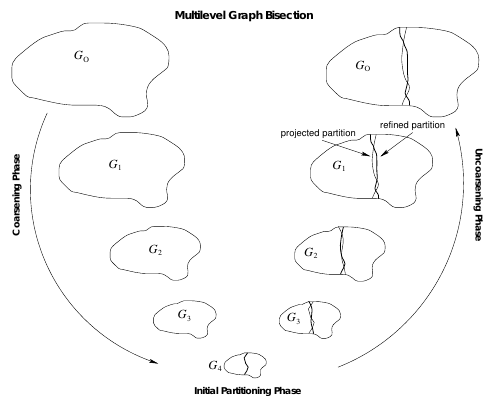
\includegraphics[keepaspectratio,width=0.6\textwidth]{img/03-graphs/multilevel.png}
                    \end{center}
                    \caption{A visualization of how the multilevel partitioning algorithm works~\autocite{karypis}.} 
                    \label{mlp-fig}
                \end{figure}
                    
                A particular implementation of Karypis and Kumar~\autocite{karypis} introduces a couple of improvements.
                A matching scheme for the coarsening stage is called heavy edge matching.
                It works by iterating over all vertices and matching each one with the vertex that is attached to the edge carrying the heaviest weight.
                This is done until all edges are matched.
                Afterward, all pairs of vertices contribute to a new vertex in a new graph, the edges of each vertex pair are aggregated and their weight is summed eventually if both nodes had an edge to the same vertex. 
                Moreover, the nodes are assigned a weight that corresponds to the number of vertices that are matched in one meta-vertex.
                The partitioning stage experiments with three different methods. The KL-algorithm~\autocite{kl}, spectral clustering~\autocite{spectral}, the graph growing partitioning algorithm --- which uses BFS with a limited number of steps from a set of arbitrarily chosen vertices.
                Finally, it proposes an improved version of the refinement procedure, where only boundary vertices are considered for interchanges between partitions.
                
                The runtime for heavy edge matching is $\mathcal{O}(|E|)$ for each level and we have at least $\mathcal{O}(\log(\frac{|V|}{|V_c|}))$ steps, where $V_c$ is the set of vertices in the coarsest graph. 
                Assuming $|V_c|$ is a small constant (in the worst-case for refinement $|V_c| = 1$), we get overall $\mathcal{O}(|E| \log(|V|))$ for the refinement procedure.
                The partitioning step is dependent on the choice of the algorithm.
                Using the KL $k$-way algorithm we have  $\mathcal{O}(k^2 \cdot |V_c|^2 \cdot \log(|V_c|)$. As $|V_c|$ is small in comparison to the original graph, this results in a reduced overall runtime complexity.
                Finally the uncoarsening including projection and refinement take $\mathcal{O}(\log(|V|) \cdot (|V_i| + \mathcal{O}(k^2 \cdot |V_i|^2 \cdot \log(|V_i|)))$ with $|V_i|$ the number of vertices in the $i$ times coarsened graph.  
                As the projection should already induce a reasonable initial partitioning the algorithm should converge quickly~\autocite{hendrickson1995multi}.
                The overall runtime depends heavily on $|V_c|$. 
                The refinement phase is the most costly step as it needs to be done for the last level too, resulting in an asymptotic complexity of $\mathcal{O}(\mathcal{O}(k^2 \cdot |V|^2 \cdot \log^2(|V|)))$.
                
            \subsubsection*{Louvain Method}\label{louvain-desc}
                The Louvain method~\autocite{blondel2008fast} is an algorithm for community detection. 
                The authors define community detection as a graph partitioning problem, where nodes within a partition shall be densely connected, while nodes belonging to different partitions shall be sparsely connected~\autocite{blondel2008fast}.
                Measuring the quality of such partitioning can be done using the modularity of the partition as introduced by Newman and Girvan~\autocite{girvan2002community}
                \[ Q = \frac{1}{2m} \sum_{u,v \in V} \left( w_{(u, v)} - \frac{w_u w_v}{2m} \right) \cdot \delta (c_u, c_v) \]
                $w_{(u,v)}$ is the weight of the edge between $u$ and $v$ (or $0$ if the edge does not exist). 
                $c_u$ and $c_v$ are the communities the respective nodes are assigned to, and $\delta$ is the Kronecker delta function, i.e. $1$ if $c_u = c_v$ and $0$ otherwise. 
                $w_u$ is the sum of the edge weights incident to $u$ and $m$ is the total edge weight $m = \frac{1}{2} \sum_{e \in E} w_e$.
                Overall the modularity is in the range $[-1, 1]$ and can be interpreted as measure for the edge (weight) density inside of a partition in contrast to the edge density in the network overall.
                
                \begin{figure}[htp]
                    \begin{center}
                        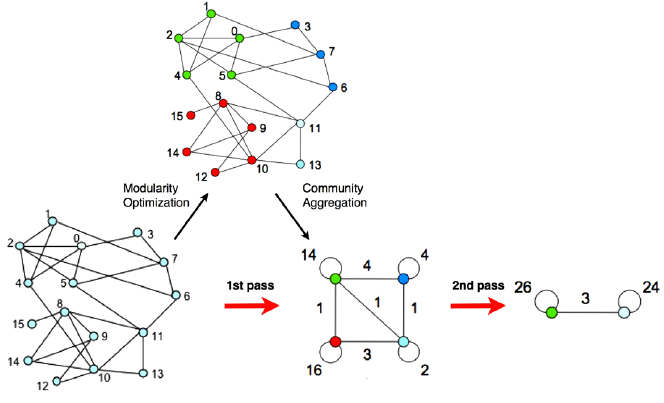
\includegraphics[keepaspectratio,width=0.6\textwidth]{img/03-graphs/louvain.png}
                    \end{center}
                    \caption{The steps that the lovain method comprises~\autocite{blondel2008fast}.} 
                    \label{louvain-fig}
                \end{figure}
                
                Optimizing the modularity exactly is computationally hard, so as soon as the graph size increases, approximate optimization is required.
                The Louvain method is such an approximation.
                Its broad control flow comprises the following steps and is visualized in Figure~\ref{louvain-fig}.
                \begin{enumerate}
                \item Initialize the initial partition with each node in an own community
                \item $\forall v \in V \forall u \in N_v:$ 
                Compute the gain in modularity $\Delta Q(u,v)$ when merging $v$ into the community of $u$. 
                Place $v$ into the community of the neighboring node $u$ where $\Delta Q(u,v)$ is maximal if the gain is positive.
                \item Go to step 2 until the improvement is below a threshold.
                \item Construct a new graph $G_i$ with the communities of the previous graph being the vertices of the new one and Aggregate the edge weights. 
                Links between nodes of the same communities are aggregated to self-loops.
                \item If the previous graph and the new graph differ, go to step 2 using the $G_i$ as input graph, else terminate.
                \end{enumerate}
                The gain in modularity is computed using a specific formulation, that eases computation
                \[ 
                  \Delta Q(v, C) = \left( \frac{I_c + 2w_{v, C}}{2m} - \left( \frac{w_C + w_v}{2m} \right)^2 \right) - \left( \frac{I_c}{2m} - \left( \frac{w_C}{2m} \right)^2 - \left( \frac{w_v}{2m} \right)^2 \right).
                \]
                Here $I_C$ is the sum of edge weights within the community $C$, $w_C$ is the sum of the edge weights incident to nodes in $C$, $w_{v, C}$ is the sum of edge weights between $v$ and nodes in $C$, $w_v$ is the sum of all edge weights incident to $v$ and $m$ is again the sum of all edge weights.
                
                Many of these quantities can be precomputed and easily updated
                $m$ is constant, $w_v$ is constant, $I_C$ can be updated by adding $w_{v, C}$, $w_C$ can be updated by adding $w_v$, only $w_{v, C}$ needs to be recomputed for every community to consider. 
                It requires iterating over all edges of $v$ and check if the other incident node is in the community, thus $\text{deg}(V)$.
                The complexity of the algorithm is determined by computing the gain in modularity for each node and its neighborhood
                $\mathcal{O}(|V| \cdot \text{deg}(V)^2)$.
                Notice, that this algorithm is similar to the coarsening phase of the multilevel algorithm.
                The contraction is done by calculating the modularity gain.
                However, not only two vertices are matched during an iteration but arbitrarily many until convergence. 
                Both partitioning and refinement are not done, as the special contraction mechanism already partitions the graph.
                That is, opposed to the top-down partitioning of the multilevel partitioning algorithm, the Louvain method works bottom-up.
                Both algorithms however generate a hierarchy.
                
                One problem with the Louvain method is its resolution limit.
                For very large and dense graphs, the total edge weight grows extremely large and thus the modularity is always small.
                This problem is approached in two different ways.
                Conde-C{\'e}spedes et al.~\autocite{conde2017comparison} experiment with different other modularity measures, that are provably stable to the graph size.
                However, those measures that provide good results require user defined-parameters, which in turn requires either domain-specific knowledge of the data or parameter optimization, which implies multiple executions of the algorithm. 
                


 

\chapter{Graph Databases}
    First, we introduce a popular data model that is employed by many current graph databases~\autocite{GitHubneo4j, ArangoDB, AmazonNeptune, RedisGraph}.
    Then we look at an implementation of this model in a native graph database called Neo4J is described. 
    The latter also serves as a role model for the implementation of the in-memory database that is used in the evaluation part.
                
    \section{Architecture}
        Graph databases, do not differ in many architectural aspects from relational and other databases. A borad sketch of the software architecture of database management systems is laid out in Section~\ref{db-arch}. 
        The most significant difference is how data is stored on the one hand side, and how the queries are evaluated on the other hand side.
        As mentioned we focus on the former issue.
        
        Relational databases store data in tables.
        The links considered in this category of DBMS are mostly used to stitch together the fields of a record stored in different tables into one row again after it has been split to satisfy a certain normal form.
        Of course one may also store tables where one table stores nodes and the other table's fields are node IDs to represent relationships.

        However, to traverse the graph, one has either to do a lot of rather expensive lookups or store auxiliary structures to speed up the lookup process.
        In particular, when using B-trees as index structure, each lookup takes $\mathcal{O}(\log(n))$ steps for clustered indices to locate a specific edge. However, as all edges are attached to two nodes, it is only possible to build a clustered index over edges either grouped by incoming or outgoing neighborhood. The undirected neighborhood permits no such sorting and retrieval as it is unclear to which node an edge is to be sorted to.
        Alternatively one could store an additional table that holds incidence lists such that the lookup of outgoing or incoming edges is only $\mathcal{O}(\log(n))$ which would speed up breadth-first traversals, but duplicate data.
        Still one has to compute joins to continue the traversal in the scope of depth first searches.
        Another way to speed things up is to use a hash-based index, but this also has a certain overhead aside from the joins and the question which hash function and which attributes to use arises.
        
        In contrast to relational databases, native graph databases use structures specialized for these kinds of queries.
            
    \section{The Property Graph Model}\label{prop-graph-model}
        The property graph model is a widely adopted data model to represent graphs in databases.
        It is not only able to represent the structure of directed or undirected, weighted or unweighted, but also of typed graphs having additional properties.

        A \textbf{Property Graph} is a 9-Tuple $G = (V, E, \lambda, P, T, L, f_P, f_T, f_L)$ with 
        \begin{itemize}
            \item $V$ the set of vertices.
            \item $E$ the set of edges.
            \item $\lambda: (V \times V) \rightarrow E$ a binary relation assigning a pair of nodes to an edge.
            \item $P$ a set of key-value pairs called properties.
            \item $T$ a set of strings used as relationship types.
            \item $L$ a set of strings used as labels.
            \item $f_P: V \cup E \rightarrow 2^P$ a binary relation that assigns a set of properties to a node or relationship.
            \item $f_T: E \rightarrow T$ a binary relation that assigns a type to a relationship.
            \item  $f_L: V \rightarrow 2^L$ a binary relation that assigns a node a set of labels.
        \end{itemize} 
        \smallskip
        The property graph model reflects a directed, node-labeled and relationship-typed multigraph $G$, where each node and relationship can hold a set of properties~\cite{angles2018property, rodriguez2012graph, Rodriguez2010ConstructionsFD}.
        In a graph, the edges are normally defined as $E \subseteq (V \times V)$, but in the property graph model edges have sets of properties and a type, which makes them records on their own. 
        An illustration of this model is shown in Figure~\ref{propertygraph}.
        
        \begin{figure}[htp]
            \begin{center}
                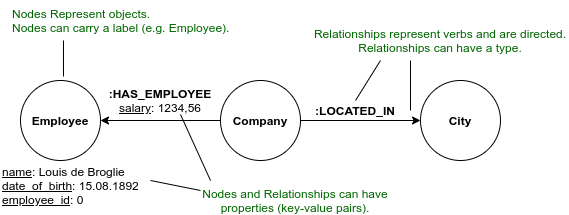
\includegraphics[keepaspectratio,width=0.6\textwidth]{img/04-databases/property_graph_elements.png}
            \end{center}
            \caption{A schematic visualization of the property graph model.} 
            \label{propertygraph}
        \end{figure}

        
        Neo4j is a graph database employing the property graph model~\cite{robinson2015graph}.
        The logical operators of this model are described in~\autocite{Holsch2016Algeb}. 
        The \textit{get\_nodes}-operator returns all nodes of the graph.
        This means that however the nodes are stored, the whole file (portion) needs to be scanned.
        Furthermore, the \textit{expand}-operator returns the incident edges of a node depending on the direction.
        Expand only considers a part of the set of all edges, so it does not do full scans but rather smaller reads.
        Finally the \textit{filter}-operand selects certain nodes or relationships based on properties, labels or, relationship type.
        
        In the next Section~\ref{n4j} we are going to discuss how Neo4J implements the property graph model, with our focus on the structure of the graph and the low-level storage scheme.

\section{Example --- Neo4J}\label{n4j}
    Neo4J is a native graph database using the property graph model.
    The source code of the community edition is available at GitHub~\autocite{GitHubneo4j}.
    We look at some implementation details of the storage and buffer manager, as well as the record structure.
    We are not going to take properties, relationship types, labels, and concepts related to those into account.
    
    \subsection{High-level Architecture}
        \begin{figure}[htp]
            \begin{center}
                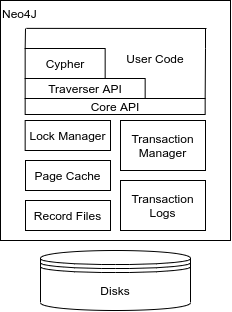
\includegraphics[keepaspectratio,width=0.25\textwidth]{img/04-databases/N4J_HLA_Emil.png}
            \end{center}
            \caption{The high level architecture of Neo4J~\autocite{robinson2015graph}.} 
            \label{N4J_HLA_Emil}
        \end{figure}
        
        To get an overview of the architecture let us consider Figure~\ref{N4J_HLA_Emil}.
        This description was outlined by the co-founder of Neo4J Emil Effrem, the chief science officer Jim Webber and Ian Robinson who was an engineer at that time at Neo4J in their book on graph databases~\autocite{robinson2015graph}.
        Here we can see that the architectural schema outlined in Section~\ref{db-arch} and especially Section~\ref{dbms_arch} was not quite applied.
        
        Still, the components are very similar.
        The ''Page Cache`` is equivalent to the buffer manager, the record files are what is managed by the disk space manager, mechanisms to deal with free slots~\autocite{neo4jidgenerator} and (de-)allocations~\autocite{neo4jio} are also part of the software stack, as are the record formats~\autocite{neo4jrecordstorage} and indexes, corresponding to the access layer. 
        The corresponding components are just put together in a slightly different manner. 
        
        \begin{figure}[htp]
            \begin{center}
                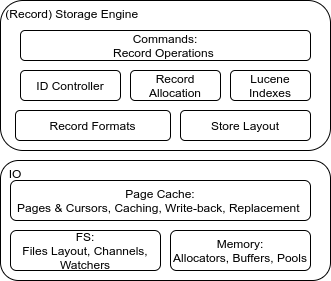
\includegraphics[keepaspectratio,width=0.33\textwidth,height=0.3\textheight]{img/04-databases/N4J_Storage.png}
            \end{center}
            \caption{A visualization of the broad storage and memory organization of Neo4J.} \label{N4J_Storage}
        \end{figure}
        
        The detailed composition is shown in Figure~\ref{N4J_Storage}.
        The IO package contains the page cache, which is the buffer manager.
        It also contains facilities to create, grow and shrink files using the \mintinline{java}{java.nio} library and wrappers around platform-dependent allocation facilities.
        Thus the (de-)allocation part of the disk space manager resides in the IO package, too.
        The record storage engine defines the record format and the file layout, as well as means to create and maintain indices, thus it is similar to the access layer. 
        It also handles the management of free slots something is usually done by the disk space manager.
        To summarize: the buffer manager and the access layer correspond closely to these two packages, while the disk space manager is distributed mainly over these two packages.        

    \subsection{Record and File Structures}\label{n4j-struct}
        Neo4J uses several different record types. They can be split broadly in the following categories:
        \begin{itemize}
            \item Variable size records: Strings, Arrays
            \item Fixed size records:
            \begin{itemize}
            \item Graph structure related records: Nodes, relationships, relationship groups
            \item Properties, labels, relationship types
            \end{itemize}
        \end{itemize}
        
        Each record type is stored in an own file per database in the database management system.
        An additional system database keeps track of the existence and metadata of the other ones storing user data.
        This is visualized in Figure~\ref{n4j-disk}.
        \begin{figure}[htp]
            \begin{center}
                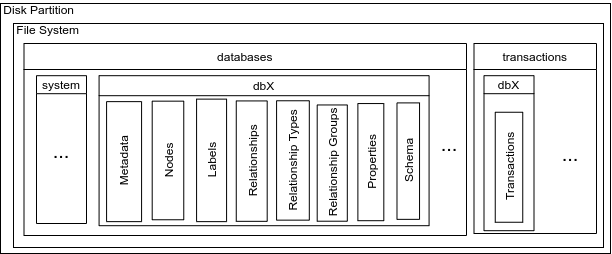
\includegraphics[keepaspectratio,height=0.4\textheight,width=0.7\textwidth]{img/04-databases/N4J_disk_view.png}
            \end{center}
            \caption{A visualization of how the files are arranged of Neo4J.}
            \label{n4j-disk}
        \end{figure}
        
        The records are ordered simply by their insertion order, i.e. the files storing the records are heap files.
        While variable-length records store strings and arrays, labels for example store a pointer to the actual string of the label to be fixed size and thus efficiently retrieved.
        The same is true for relationship types and property keys and values that are strings or arrays.
        This is done to avoid duplications of strings e.g. of each label.
        As mentioned before for the sake of succinctness we are just going to elaborate on the elements that represent the graph structure. 
        Only one thing is to be mentioned.
        Properties are stored as a linked lists for each node and relationship.
        
    \subsubsection*{Node Records}
        \begin{figure}[htp]
            \begin{center}
                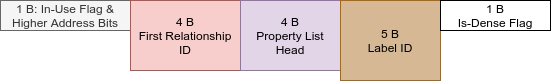
\includegraphics[keepaspectratio,height=0.4\textheight,width=0.7\textwidth]{img/04-databases/node_record.png}
            \end{center}
            \caption{A visualization of the record structure of a node record~\autocite{neo4jNodeRecordFormat}.}
            \label{node-record-format}
        \end{figure}
        The record format of nodes consists of a 15-byte structure.
        The IDs of nodes are stored implicitly as their address.
        If a node has ID 100 we know that its record starts at offset $15 \text{ Bytes} \cdot 100 = 1500$ from the beginning of the file.
        The struct of a record is outlined below.
        \begin{enumerate}
            \item Byte 1: One bit for the in-use flag. 
            The additional bits are used to compress the node struct by using the other 7 bits to store the most significant bits of the first relationship ID and the first property ID 
            \item Bytes 2 --- 5: The next 4 Bytes represent the relationship ID of the head in the linked list of relationships of the considered node.
            \item Bytes 6 --- 9: Again 4 bytes encode the property ID of the head in the linked list of properties of the node.
            \item Bytes 10 --- 14: This 5-byte section points to the labels of this node.
            \item Byte 15: The last byte stores if the node is dense, i.e.\ has an awful lot of relationships, such that it needs special treatment to remain efficient to traverse over.
            That is, relationships are grouped by type, and direction for this node.
        \end{enumerate}
        
        To summarize: the records on disk are stored as in the enumeration above, and as shown in Figure~\ref{node-record-format}. 
        In the database all IDs get mapped to longs, and their respective space is larger than the space representable by 35 bits --- which is perfectly fine.
        
        On-disk 4-byte integers are used to store the 32 lowest bits of the respective addresses and the higher bits are stored in the first byte that also carries the in-use bit.
    
    \subsubsection*{Relationship Records}\label{n4j-rel}
        \begin{figure}[htp]
            \begin{center}
                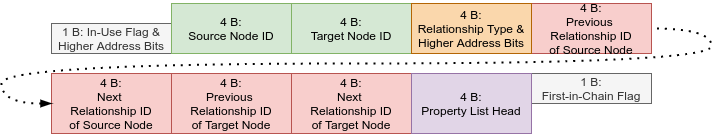
\includegraphics[keepaspectratio,height=0.9\textheight,width=0.9\textwidth]{img/04-databases/relationship_record.png}
            \end{center}
            \caption{A visualization of the record structure of a relationship in Neo4J.}
            \label{rel_record}
        \end{figure}
            
        Relationship records are stored with implicit IDs too. 
        Their fixed-size records contain 34 bytes.
        Besides an in-use flag, the source and target node IDs, and the relationship type, the record also contains two doubly linked list.
        One for the incident edges of the source node and one for the incident edges of the target node.
        Next, a link to the head of the linked list of properties for this relationship is stored.
        Finally, the last byte contains a marker if this relationship is the first element in the incidence list of one of the nodes.
        
        \begin{enumerate}
            \item Byte 1: In-use bit, source node high order bits (3 bits), first property high order bits (4 bits)
            \item Bytes 2 --- 5: source node ID 
            \item Bytes 6 --- 9: target node ID 
            \item Bytes 10 --- 13: relationship type (16 bit), target node high order bits (3 bits), relationship previous and next ID higher bits for source and target node ($4 \cdot 3 = 12$ bits), one unused bit.
            \item Bytes 14 --- 17: previous relationship ID the for source node
            \item Bytes 18 --- 21: next relationship ID for the source node
            \item Bytes 22 --- 25: previous relationship ID for the target node
            \item Bytes 26 --- 29: next relationship ID for the target node
            \item Bytes 30 --- 33: link to the first property of the relationship
            \item Bytes 34: A marker if this relation is the first element in the relationship linked list of one of the nodes stored in the lowest two bits of the byte. 
            The other 6 bits are unused.
        \end{enumerate}
        
        \begin{figure}[htp]
            \begin{center}
                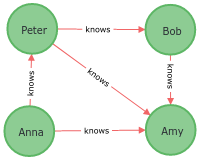
\includegraphics[keepaspectratio,height=0.4\textheight,width=0.3\textwidth]{img/04-databases/graph.png}
            \end{center}
            \caption{An example graph.}
            \label{n4j-ex-gr}
        \end{figure}
        
        The relationship structure is a key element of the layout and reveals the actual data type that the database is using.
        Nodes and relationships are both stored once only (i.e. nothing is duplicated).
        Without taking the fields into account, this is an unordered edge list.
        When taking the linked lists of relationships into account, it turns out that the underlying data structure is that of an incidence list, with a couple of additional properties.
        
        First, as already mentioned, the edges are not physically duplicated but only referenced. 
        The records are fixed-sized, so addressing them is done by multiplying the index by the size of an entry, meaning one does not need to store primary keys explicitly, and address translation can be done using simple multiplication. 
        Theoretically one could align the record size to a power of two to turn the multiplication into a bit shift.
        Next, as doubly linked lists are used, the deletion of an edge is in $\mathcal{O}(1)$ if the ID is known.
        If this was not the case, the incidence list would need to be traversed to find the previous element.
        Also, the incidence list is stored in the relationships.
        Thus to traverse from one node's incidence list to another, there is no need to load the node record itself.
        It suffices to just dereference the next element in the incidence list stored by the relationships, along with storing the ID of the edge that started the traversal.
        This makes the assumption, that the doubly linked incidence lists are circular, i.e. the head's pervious element is the tail and reciprocally.

        To conclude this example, we briefly visualize the just described storage schema. 
        The high-level graph is shown in Figure~\ref{n4j-ex-gr}.
        It contains four nodes and five edges.
        The underlying instantiated data structures are shown in Figure~\ref{n4j-ex}.
        The light red arcs represent edges, the light green circles represent nodes.
        The colored boxes on the edges and nodes represent the data structures.
        The brighter red edges represent the doubly linked incidence lists.
        Notice, that the heads and tails of the doubly linked incidence lists are marked by ''X`` to avoid drawing additional edges.
        The brighter green arrows represent the source and target nodes, as stored by the edges.
        \vfill
        \begin{figure}[htp]
            \begin{center}
                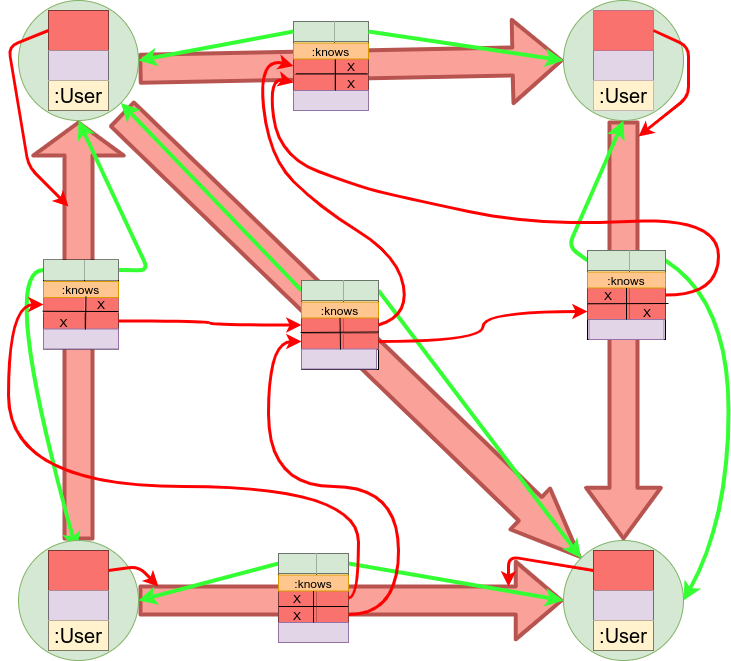
\includegraphics[keepaspectratio,height=\textheight,width=\textwidth]{img/04-databases/example_structs.png}
            \end{center}
            \caption{Visualization of the data structures, as initialized by the example graph shown in Figure~\ref{n4j-ex-gr}.}
            \label{n4j-ex}
        \end{figure}
        \vfill

\chapter{Problem Definition}\label{\positionnumber}
\section{Locality}\label{\positionnumber}
    The memory hierarchy tries to unify the strengths of fast, low capacity memory --- caches (SRAM) ---, with slower but larger memory --- main memory (DRAM), with orders of magnitude slower but orders of magnitude larger memory --- disks (HDD) and more recently flash memory (SSD, SD-Cards).
    But how can this work? 
    Given that only a tiny fraction of fast memory is available to hold the necessary parts, while additional loads of data are transferred in time --- ``desirably fast enough''.
    
    The key principle for the memory hierarchy to work is what is called \textit{locality of reference} in the literature~\autocite{jacob2010memory, tanenbaum2015modern}. 
    This principle expresses, that most programs do not access their address space uniformly or randomly, but rather tend to access small subsets of all addresses in certain time intervals, depending on the program state.
    Locality can be approached in two ways~\autocite{denning2006locality}: 
    
    \begin{itemize}
     \item \textit{Temporal locality} refers to the number of other references between two accesses of the same memory location. 
     \item \textit{Spatial locality} refers to the number of accesses and the radius of the neighborhood that is accessed in several steps.
    \end{itemize}
    
    If the same location is accessed multiple times in a short amount of time, the temporal locality is high.
    Thus temporal locality can be measured using reference frequencies.
    From a Bayesian point of view, one can say that temporal locality is the probability of an object being re-referenced after the first usage~\autocite{gupta2013locality}. 
    \[ P (X_{t + \Delta} = A | X_t = A) \]
    $X_t$ is the reference at time step $t$, $A$ is an address and $\Delta$ is a parameter, which depends not only on the system specifications (like the CPU and memory clock) but also on the program and the scale of interest.
    
    If a small range of addresses is accessed very often then spatial locality is high.
    If the range is limited to one address, then spatial locality is equivalent to temporal locality. Thus temporal locality is a special case of temporal locality~\autocite{gupta2013locality}.
    With $\varepsilon$ a radius we can characterize spatial locality by:
    \[ P(X_{t + \Delta} = A \pm \varepsilon | X_t = A) \]
    Spatial locality is thus a function of time $\Delta$ and neighborhood range $\varepsilon$. 
    
    To leverage these concepts, several components profile the memory usage.
    In the memory hierarchy, all on and off-chip caches (i.e. SRAM) are handled by hardware~\autocite{jacob2010memory}.
    
    At the level of main memory (DRAM), the operating system manages what is fetched, buffered, and evicted from disk to main memory. 
    The optimal buffering strategy is to load what is needed before its usage and evict the objects whose usage is furthest in the future~\autocite{tanenbaum2015modern}. 
    
    When it comes to eviction the best approximation to the optimal strategy is the least recently used algorithm. 
    It aims to keep things in memory, that have the highest chance to exhibit temporal locality.
    That is, the things in memory, that have not been referenced for the longest time, have a lower chance to be temporally local in the future~\autocite{silberschatz2006operating}.
    Put differently \textit{caches and buffers exploit temporal locality}.
    
    As this information is not available in general, objects are loaded when they are referenced, often with additional addresses which are hoped to be needed, too --- this is called prefetch or predictive fetching~\autocite{stallings2012operating, jacob2010memory}. 
    Prefetch tries to exploit spatial locality. Several components try to exploit this:
    \begin{itemize}
     \item Compiler-generated prefetches: 
     The compiler knows what addresses the program accesses in which sequence and tries to minimize the time that is spent waiting for IO. 
     This is called instruction scheduling~\autocite{aho1986compilers}. 
     Other compiler-generated heuristics are applied e.g. in domain-specific compilers, like in the TVM compiler for neural networks~\autocite{chen2018tvm}.
     
     \item The operating system may use specialized data structures and algorithms to estimate, if prefetching should be done, based on the previous accesses. 
     An example is the ``spatial look-ahead'' algorithm by Baier and Sager~\autocite{jacob2010memory, baier1976dynamic}, but there exist many more e.g. \autocite{joseph1999prefetching, griffioen1994reducing, kroeger1997exploring, cooksey2002stateless}. 
     Most of these methods are capable to find correlations between addresses and their neighborhood, file accesses, and pointed-to objects.
     
     \item A special role in the context of prefetches and spatial locality take databases. 
     As these are not only able to predict content-based correlations, e.g. by knowing what table is queried in the case of relational databases, but also can augment data by using auxiliary data structures like indices. 
     The most remarkable capability in this context is to be able to reorganize data, based upon how it is queried.
     Relational databases store data in tables and often sort these tables based upon either a certain field (like the primary key) or a set of fields. 
     This in combination with being able to analyze the query before executing it allows reordering the memory accesses, such that as many accesses as possible are sequential~\autocite{ramakrishnan2000database, silberschatz1997database}.
    \end{itemize}
    
    Spatial locality depends on how data is ordered:
    If semantically closely coupled data is spread out as wide as possible, the program or file of interest will hardly exhibit locality. 
    As an example consider a program with $n$ instructions, with logical addresses from $0, \dots, n-1$. 
    An inversion is a change of position of two lines $l_1, l_2$, such that the line that gets executed earlier $l_1$ has a higher address than one that gets executed later $l_2$.
    Such a program can maximally have $\frac{n (n-1)}{2}$ inversions. 
    If it has that many inversions, the program is laid out in the opposite direction and the spatial locality would be similar to the original program.
    Thus let us assume only every second instruction is misplaced. 
    In effect, to execute the program two pages must always remain in memory instead of one, and the radius of the neighborhood doubles.
    
    In short, the layout of the data or records in the address space --- on file or in memory --- is crucial to the concept of spatial locality. 
    Achieving optimal temporal locality is a matter of grouping and ordering data such that what is referenced together is in a neighborhood in terms of addressing.
    
          
\section{Problem Definition}\label{prob-def}
    To optimize spatial locality for traversal-based queries, the graph needs to be grouped and ordered.
    Ultimately disk storage and IO is block-based and disk access is page-based. 
    That is the vertices and edges must be grouped into blocks.
    This can happen statically or dynamically. 
    We focus here on the static reordering.
    That is the underlying data is stored only on request.
    
    \paragraph{Assumptions:}
    In the remainder of this thesis, we are assuming that the graph is represented in the property graph model Section~\ref{prop-graph-model} and uses incidence lists (see Section~\ref{inci}) as the storage schema. 
    We are not taking properties, labels, and relationship types into account.
    We are focusing on spatial locality here, that is the page replacement algorithm is fixed but arbitrary.
    Finally in the remainder of the thesis when talking about traversal-based queries, we mean all queries described in Section~\ref{queries}, but the random walk.
    
    \paragraph{Problem Definition:} Given a graph $G$, logical block size $b$, page size $p$. \\
    Desired is 
    \begin{enumerate}
     \item A partition of $G$ into blocks of vertex records $V_i$ and $E_i$ relationship records, 
     \item orderings or permutations $\pi_v, \pi_e$ of the blocks of vertex and edge records $V_i, E_i$,
     \item a reordering of the incidence list pointers
    \end{enumerate}
    such that spatial locality is as high as possible for traversal-based queries.
    
    As partitioning a graph optimally~\autocite{andreev2006balanced}, as well as finding an optimal linear arrangement~\autocite{garey1974some} are both NP-complete problems~\autocite{lewis1983computers}, we use the formulation ``as high as possible'' instead of optimal or maximal.
    
    To measure the spatial locality we introduce two measures that are used in the evaluation chapter:
    \begin{enumerate}
     \item Number of block accesses.
     \item Number of non-consecutive block accesses.
    \end{enumerate}
    The first measure is to take the locality within a block into account:
    If those vertices and edges that are accessed together are stored in the same block, this measure should be as small as possible.
    The second measure takes the order of the blocks into account: 
    If vertices and edges that are connected or ``close'' to each other are stored in adjacent blocks, they can be loaded with one sequential read.
    But the second measure also takes into account how the traversal is executed in terms of pointer chasing concerning the incidence list.
    
    As we change the unit of access from addresses of records to blocks on a disk, the definition of locality needs to be adapted.
    Temporal locality is now based on blocks instead of addresses.
     \[ P (X_{t + \Delta} = B | X_t = B) \]
     Here we have a block $B$ instead of an address $A$. 
     If blocks are well-formed, the number of blocks that are accessed should decrease overall.
     This is because those multiple elements that are accessed in a short amount of time are stored in the same block instead of several. \\
     Spatial locality can be reformulated in the same sense:
      \[ P(X_{t + \Delta} = B \pm \varepsilon | X_t = B) \]
      With a well-suited ordering of the blocks, the probability that neighboring blocks are accessed should be increased.
      Finally, when the incidence list is ordered, the access to blocks should be in a monotone increasing sequence of block addresses. 
      Thus the access should be sequential and thus the probability to access adjacent blocks increases as opposed to unordered access that jumps back and forth.
    
\section{Example: Vertex, Edge and Incidence List Order}
  Why are these three criteria necessary? Why are there only two measurements for three criteria? \\
  This is what shall be explained in an example.
  Something that is of importance for the traversal --- but not as straightforward to see as anode and edge grouping and order --- is the order of the pointers in the incidence list, as we are going to see.
  
  \begin{figure}[htp]
    \begin{center}
        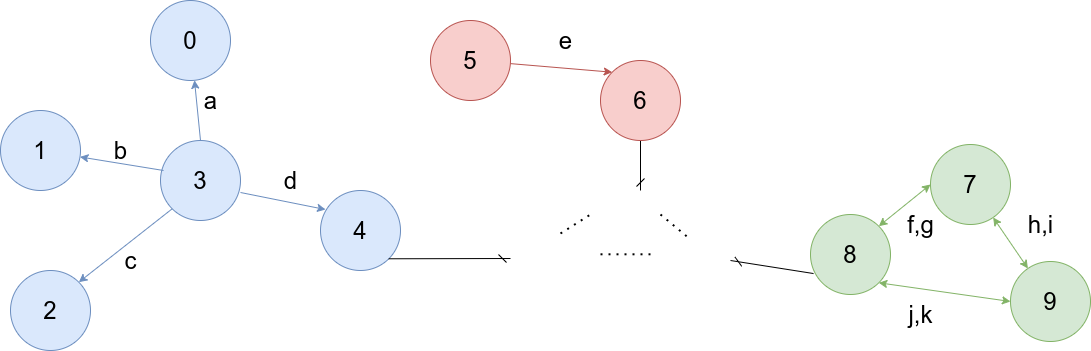
\includegraphics[keepaspectratio,height=0.3\textheight,width=\textwidth]{img/05-problem_def/example_graph.png}
    \end{center}
    \caption{Parts of a graph that is used in subsequent examples. Cut through edges mean edges to any non-visualized component of the graph. The dotted lines indicate, that other nodes and edges are between the three shown components.}
    \label{ex-gr}
  \end{figure}
  
  The graph used in the below example looks as shown in Figure~\ref{ex-gr}.
  We use a storage schema that is motivated by the one of Neo4J.
  Nodes and relationships are stored in separated files, the incidence list is stored in the records of the edges and the nodes contain a pointer to the head relationship of their incidence list each. 
  Moreover, we assume that we can only read sequentially if the blocks are adjacent.
  As this is a rather small example for the sake of succinctness, things are just shown on a conceptual level. 
  We assume that 3 nodes or 2 relationships fit onto a disk block. 
  Realistically 8 to 16 nodes and 5 to 8 relationships fit on a 512-byte disk block. 
  An average graph in the Stanford network analysis platform graph dataset collection has thousands of nodes and edges. 
  Taking the californian road network graph as an example, the whole graph would take 
  \[ 1 965 206 \text{ nodes} \cdot 35 \text{ bytes per node} \cdot 512^{-1} \text{ bytes per block} = 134 341\text{ blocks}\] 
  to store all nodes and 
  \[2 766 607 \text{ relationships} \cdot 72 \text{ bytes per relationship} \cdot 512^{-1} \text{ bytes per block} = 389055\text{ blocks}\] 
  blocks to store the relationships in Neo4J.
  To summarize, the principles shown below scale with the graph size and for realistic assumptions, these conditions emerge.

  First, consider the split of vertices and edges into blocks in the upper half of Table~\ref{blocks}. 
  None of the vertices in the blocks are neighboring each other.
  Thus when traversing the graph, each step requires to load a block.
  The same is true for the edges: 
  None of the edges in the same block are connected to the same vertex. 
  Each edge causes a page fault and a load of another block(s).
  This may happen in current state-of-the-art graph databases like Neo4J. 
  The placement into blocks is currently by insertion order, thus depends on the ordering of the input dataset. 
  On the other hand side in the lower half of Table~\ref{blocks}, the vertices are grouped into blocks according to their neighborhood and the edges are grouped by the vertices they are connected to.

  
     \begin{table}[htp]
     \centering
    \begin{tabular}[c]{|l|c|c|c|c|c|c|} \hline
    &&&&&&\\[-1em]
     node.db & \colorbox{blue!30}{0}, \colorbox{red!30}{5}, \colorbox{green!30}{7} & \colorbox{blue!30}{1}, \colorbox{blue!30}{4}, \colorbox{green!30}{9} & \colorbox{blue!30}{2}, \colorbox{red!30}{6}, \colorbox{green!30}{8} & \colorbox{blue!30}{3} &  & \\ \hline
     &&&&&&\\[-1em]
     edge.db & \colorbox{blue!30}{a}, \colorbox{green!30}{f} & \colorbox{blue!30}{b}, \colorbox{green!30}{g} & \colorbox{blue!30}{c}, \colorbox{green!30}{h} & \colorbox{blue!30}{d}, \colorbox{green!30}{i} & \colorbox{red!30}{e}, \colorbox{green!30}{j} & \colorbox{green!30}{k} \\  \hline
    \end{tabular}
    \vspace{0.5cm}
    
    \begin{tabular}{|l | c | c | c | c | c | c|} \hline
    &&&&&&\\[-1em]
     node.db & \colorbox{green!30}{7},\colorbox{green!30}{8}, \colorbox{green!30}{9} & \colorbox{blue!30}{0}, \colorbox{blue!30}{1}, \colorbox{blue!30}{3} & \colorbox{red!30}{6} & \colorbox{blue!30}{4}, \colorbox{blue!30}{2}, \colorbox{red!30}{5},  &  & \\ \hline
     &&&&&&\\[-1em]
     edge.db &  \colorbox{green!30}{f}, \colorbox{green!30}{h} & \colorbox{green!30}{g}, \colorbox{green!30}{k} & \colorbox{green!30}{i}, \colorbox{green!30}{j} & \colorbox{blue!30}{a}, \colorbox{blue!30}{b} & \colorbox{red!30}{e} & \colorbox{blue!30}{c}, \colorbox{blue!30}{d} \\ \hline
    \end{tabular}
  \caption{An example of suboptimal and improved record placement into blocks. 
  The block size is assumed to be only 3 vertex records and 2 node records respectively. 
  For larger block size, the same principle applies.}
   \label{blocks}
   \end{table}
    
  Next, Table~\ref{order} shows two different orderings of the blocks, this time with a focus on the edges only. 
  In the upper table, an edge is stored in the neighborhood of its source node but far apart from its target node.
  Thus two single reads are required to go from one vertex over an edge to another vertex and retrieve its incident edges. 
  In the lower table, the blocks are adjacent and one sequential read is enough to go from source to target and fetch the target's incidence list.
  
     \begin{table}[htp]
          \centering
    \begin{tabular}{|l | c | c | c | c | c | c|} \hline
    &&&&&&\\[-1em]
     edge.db &  \colorbox{green!30}{f}, \colorbox{green!30}{h}   & \colorbox{blue!30}{a}, \colorbox{blue!30}{b} & \colorbox{green!30}{i}, \colorbox{green!30}{j} & \colorbox{red!30}{e} & \colorbox{blue!30}{c}, \colorbox{blue!30}{d} & \colorbox{green!30}{g}, \colorbox{green!30}{k} \\ \hline
    \end{tabular}
    \vspace{0.5cm}
    
    \begin{tabular}{|l | c | c | c | c | c | c|}\hline
    &&&&&&\\[-1em]
     edge.db &  \colorbox{green!30}{f}, \colorbox{green!30}{h} & \colorbox{green!30}{g}, \colorbox{green!30}{k} & \colorbox{green!30}{i}, \colorbox{green!30}{j} & \colorbox{blue!30}{a}, \colorbox{blue!30}{b} & \colorbox{blue!30}{c}, \colorbox{blue!30}{d} & \colorbox{red!30}{e} \\ \hline
    \end{tabular}
      \caption{Suboptimal and improved block order.}
    \label{order}
       \end{table}
  
  Finally, consider the visualization of the incidence list of node 3, given the page placement in the upper part of Table~\ref{blocks} and Table~\ref{inc-ord}. 
  Theoretically, the only difference is the order in which the list points to the relationships. 
  In terms of traversed blocks, we need to do four single reads when using the order given in the upper table. 
  If we rearrange the pointers according to the lower table, the list may be loaded sequentially with one read operation instead of four single reads. 
  This phenomenon may also appear when the blocks are formed and ordered in an improved way, but only when scaling up to a graph with larger neighborhoods.
  Given that an edge can be placed either near the other edges of the source or the target node, the impact when jumping back and forth will grow along with the gaps between blocks in which the edges are stored.
  Finally, if the blocks are cached, this induces a higher load on the buffer manager, as more pages need to reside in memory at the same time and as they are frequently re-referenced instead of being read once and evicted then.
  The higher the degree --- i.e. the length of the incidence list --- of the node, the more severe the effect.
  % TODO validate!

\begin{table}[htp]
          \centering
    \begin{tabular}{|l | c | c | c | c |}\hline
     incidence list of node 3 &  c & a & d & b\\ \hline
    \end{tabular}
    \vspace{0.5cm}
    
    \begin{tabular}{|l | c | c | c | c |}\hline
     incidence list for node 3 &  a & b & c & d\\ \hline
    \end{tabular}
      \caption{Suboptimal and improved incidence list order.}
    \label{inc-ord}
\end{table}

\chapter{Locality-optimizing Static Record Layout}
\section{G-Store: Multilevel Partitioning}
    G-Store is a disk-based storage manager for graph data implemented and published by Steinhaus et al.~\autocite{steinhaus2010g}. 
    To the best of the author's knowledge, this is the first structured approach to improve locality in graph databases by altering the placement of records into blocks.
    More specifically, to maximize performance, they try to place adjacent nodes close to each other, such that they can be read sequentially. 
    The rearrangement of the records is done when importing a new data set and is static after insertion.
    G-Store uses an adjacency list as the data structure and does not store these in an own file but directly next to the vertex in the very same file.
    The broad schema of the placement method developed by Steinhaus et al.~\autocite{steinhaus2010g} is derived from multilevel partitioning methods, that is described in Section~\ref{mlp}.
    Briefly, the multilevel partitioning algorithm works in three steps: coarsening, turn-around, and uncoarsening. 
    The coarsening phase tries to reduce the original graph to a smaller one that broadly preserves the structure of the underlying graph. 
    A more expensive partitioning algorithm can then be applied to this smaller graph to solve the actual problem approximately and fast.
    During the uncoarsening, the approximate solution is refined and the coarser graph is projected back until the original graph is mapped and restored.
    Finally, in the last step, the partitions are mapped to actual blocks.
    Note how similar the procedure is to the actual multilevel partitioning algorithm. 
    Thus we are more interested here in the differences from the reference algorithm.
    A broad overview of the method is shown in Figure~\ref{g-store}.
    
    \begin{figure}[htp]
        \begin{center}
            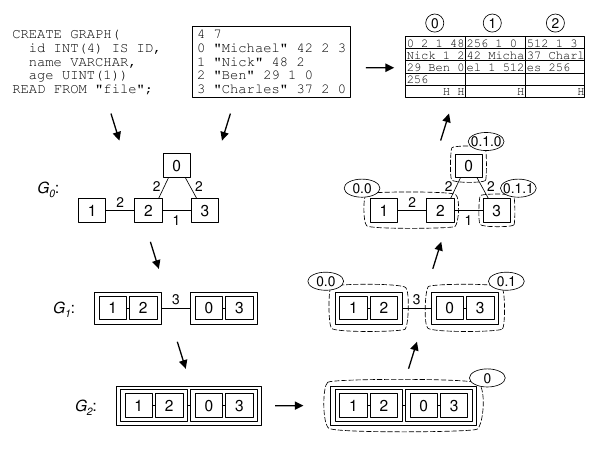
\includegraphics[keepaspectratio,width=0.7\textwidth]{img/06-rel_w/g-store.png}
        \end{center}
        \caption{A broad overview of the multilevel partitioning method applied by G-Store~\autocite{steinhaus2010g}.} 
        \label{g-store}
    \end{figure}

    
    In the next part of this section, we are going to use the notions of a finer and a coarser graph a lot. Let therefore $G = G_0 = (V_0, E_0)$ the original graph, and $G_i = (V_i, E_i)$ the graph that was coarsened $i$ times.
    
    \subsection*{Coarsening}
    The coarsening phase of G-Store's partitioning algorithm is what is called heavy edge matching (HEM) in Karypis formulation of the algorithm as already mentioned. 
    Thus the algorithm takes $G_i$ as an argument and returns $G_{i+1}$ along with a projection $Z_{i+1}$ specifying which finer nodes map to which coarser node.
    Coarsening proceeds in the original algorithm until a certain lower limit of vertices is reached.
    In the METIS implementation this is hard-coded to  $\max \left( 20k, 40 \log_2 k\right)$ where $k$ is a user defined parameter specifying the number of partitions.
    The algorithm used in G-Store keeps coarsening until there are no edges, i.e. only one vertex.
    It can thus be seen as a form of hierarchical agglomerative clustering~\autocite{hac} with the inverse edge weight acting as a distance function.
    
    Another modification is that in contrast to METIS~\autocite{karypis}, not only two edges are matched at a time but possibly many and that there is an upper limit to the vertex weights. 
    This depends on the coarsening factor $c(i) = \frac{|V_i| - |V_{i+1}|}{|V_i| - |\{v \in V | N_v = \emptyset \}|}$, with $i$ the level of coarsening, where $i=0$ it the original graph.
    The counter is the number of vertices that were reduced and the denominator is the number of nodes in the larger graph minus the irreducible nodes.
    Initially, the allowed vertex weight $\theta$ is the size of a block.
    If this factor $c(i) < 0.3$ then the node weight $\theta$ is doubled as long as $\theta \leq 32$.
    Otherwise, the number of nodes that are allowed to be matched is incremented.
        
    \subsection*{Turn-Around}
    In G-Store the turn-around simply assigns every vertex in the coarsest graph, whose weight is larger than the size of a block, a distinct partition number.
    The other nodes are added up until their weight reaches the size of a block and are assigned a partition number together.
    Thus the algorithm accepts a fully coarsened graph $G_i$ and returns the partition numbers for this graph $\phi_i$.
    
    This step is completely different than in the reference multilevel partitioning algorithm.

    
    \subsection*{Uncoarsening}
    The uncoarsening phase consists of three different steps that are performed per level:
    projection, reordering, and refinement.
    Projection constructs the first mapping, reordering swaps partitions, and refinement exchanges nodes between partitions.
    Each iteration of the full uncoarsening procedure takes the coarser graph $G_{i+1}$ as an argument along with its the partition numbers $\phi_{i+1}$ and the mapping $Z_{i}$ and returns the one level uncoarsened graph $G_i$, along with the respective partition numbers $\phi_i$.
    The algorithm also defines a weight threshold per level. With $\overline{c}$ the average coarsening factor
    \[ \chi_i = \lfloor \frac{\text{block size}}{(1-\overline{c})^i} \rfloor. \]
    
    Further, it defines three objective functions:\\
    The first function is closesly related to the minimal linear arrangement problem~\autocite{lewis1983computers} and expresses that nodes that share an edge shall be minimally far appart from each other.
    \[ \min C_1 = \min \sum_{(u,v) \in E} |\phi(u) - \phi(v)| \]
    The second objective function aims to reduce the overall number of edges between the partitions.
    \[\min C_2 = \min \sum_{(u,v) \in E)} \begin{cases}
        1 & \phi(u) \neq \phi(v) \\
        0 & \text{ otherwise}
    \end{cases}
\]
    The last objective function penalizes the number of blocks that are linked. That is to reduce the number of overall linked blocks according to~\autocite{steinhaus2010g}.
    \[ \min C_3 = \min \sum_{i \leq j} 
    \begin{cases}
        1 & \phi(u) = i \wedge \phi(v) = j, \ (u,v) \in E \\
        0 & \text{ otherwise}
    \end{cases}
    \]
    
    Finally there are two functions that are similar to the first objective function that are used in the projection step called tension and modified tension:
    The tension is the weighted distance between the block of the vertices that share and edge. Let $v \in V_i$.
    \[ t(v) = \sum_{u \in N_v} w_{(u,v)} \phi_i(v) - \phi_i(u)\]
     The modified tension is just the same, but instead of using the actual graph, one uses the coarser graph $G_{i+1}$ and the projection $Z_{i}$ to estimate the tension:
     \[ t'(v) = \sum_{u \in N_v} w_{(u, v)} \phi_{i+1}(Z(v)) - \phi_{i+1}(Z(u)) \]
    
        \subsubsection*{Projection}
        This part of the algorithm constructs a first version of the finer-grained partition numbers $\phi_i$ from the coarser ones $\phi_{i + 1}$.
        The enumeration follows a Dewey numbering scheme~\autocite{dewey1894decimal}.
        That is per level one place in the partition label is added. 
        If the vertex $\phi_{i+1}(Z(v)) = 2$ and vertex $\phi_i(v) = 1$, then the overall partition label of the vertex is $2\text{.}1$. 
        
        Per partition in the coarser level graph, the algorithm either simply assigns the same partition number to all nodes $v_i \in Z(\phi{i+1,j})$ in the finer graph $G_i$ that were clustered into the respective coarser nodes, if the overall weight of the partition in the coarser graph is smaller than the weight threshold: $w_{\phi{i+1, j}} \leq \chi_i$.
        Otherwise the modified tension is computed for all nodes of the partition in the finer graph $\forall v_i \in Z(\phi{i+1,j}): t'(v_i)$.
        The minimal tension is extracted, placed to the leftmost free position in the partition and the tensions of the neighbors are updated. 
        This is done repeatedly until all nodes are placed.
        During this step, each partition is marked with a flag, which is true when it was created from nodes in the right half of the coarser partition.
        
        The projection differs vastly from the reference algorithm that just assigns the coarser partition number to all nodes in the finer-grained graph.
                
        \subsubsection*{Reordering}
        This step is non-existent in the multilevel partitioning algorithm.
        When swapping the above created partitions, only $C_1$ changes, but not $C_2$ or $C_3$. Using the just created flags, groups are identified which span two half coarser partitions $\phi_{i+1,j}, \phi_{i+1,j+1}$. Per group, the finer partitions are swapped as long as the overall absolute tension ($C_1$) decreases by some swap.
        In effect, this is a fix-point computation.
        
        \subsubsection*{Refinement}
        Finally, the refinement step tries to optimize a weighted sum of all the objective functions by moving vertices to other partitions.
        In the reference algorithm, this step simply uses the gain as defined in Section~\ref{kla}.
        Three used-defined parameters $\alpha, \beta, \gamma$ control the weighting, another one specifies the number of iterations that shall be executed $r$.
        In each iteration, the algorithm steps over the partitions $\phi_{i,j}$ and creates a two dimensional array $A$ of dimension $|\phi_{i,j}| \times |P_{i,j}|$ with $P_{i,j} = \{ \phi_i(u) | v \in \phi_{i,j}, u \in N_n\} \setminus \phi_{i,j}$.
        Each entry is defined with $v$ the vertex that is to be moved to partition $k$:
        \[ a_{v,k} = \alpha C_1 + \beta C_2 + \gamma C_3 + \lambda \]
        Where $\lambda$ penalizes overfull blocks or rewards the filling of less filled blocks.


    
\section{ICBL: Diffusion Set-based Clustering}
    Ya\c{c}ar and Gedik propose another method to form and order blocks~\autocite{yacsar2015scalable, yacsar2017distributed}. 
        
    They define one metric for each of the task:
    \textit{Block locality} is defined by the means of conductance and cohesiveness. 
    Conductance is defined as the ratio of edge cuts to total edges in a block:
    \[ C_d (B) = \frac{|\{ (u,v) \in E: |\{u,v\} \cap V_B| = 1\}|}{|\{ (u,v) \in E: |\{u,v\} \cap V_B| > 0\}|} \]
    Cohesiveness is the number of nodes in the same blocks that are connected by an edge divided by the number of theoretically possible edges, i.e. $|V|^2$ in a directed graph. The authors assume an undirected self-loop free graph, thus the number of possible edges is $\frac{|V| (|V| - 1)}{2}$.
    \[ C_h (B) = \frac{|\{ (u,v) \in E: u,v \in V_B \}|}{|V|^2} \]
    As conductance takes edges between blocks into account and cohesiveness measures the edges within a block, they are complementary~\autocite{yacsar2015scalable}.
    Thus the locality of a block us defined as the geometric mean of the measures above, where the conductance is subtracted from one:
    \[ L(B) = \sqrt{C_h (B) \cdot (1 - C_d (B))} \]
    \textit{Ranking locality} is related to what we called tension before. 
    Here we do not measure it between partitions of the node but directly to the position in the order. 
    Let $v \in V$ a node and $r(v)$ a function that assigns a natural number in the range of $\{0, \dots, |V|-1\}$ to each vertex.
    \[ R (v) = \sum_{u \in N_v} r(v) - r(u) \]
    The locality of a block is then defined by one minus the normalized average distance for all vertices in the block:
    \[ R(B) = 1 - \frac{1}{(|V| - 1)} \sum_{v \in V_B} \frac{R(v)}{|N_v|} \]
    
    \begin{figure}[htp]
        \begin{center}
            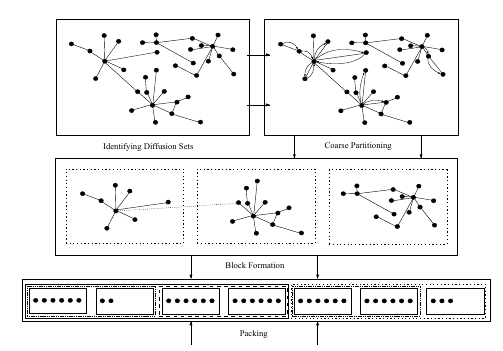
\includegraphics[keepaspectratio,width=0.8\textwidth]{img/06-rel_w/icbl.png}
        \end{center}
        \caption{A broad overview of the ICBL method by Ya\c{c}ar and Gedik~\autocite{yacsar2015scalable}.} 
        \label{icbl}
    \end{figure}

    ICBL is an acronym for the single steps performed by this algorithm. 
    It is designed to be implemented and executed using the map-reduce model.
    First ICBL extracts so-called diffusion sets as features.
    Then it clusters the vertices based upon these features, to split the graph into subgraphs.
    After that, it hierarchically clusters the subgraphs obtained in the previous step to form blocks.
    Finally, the just-formed blocks are ranked and laid out on disk.
    A brief visualization of the method is shown in Figure~\ref{icbl}.
    
    \subsection*{Identify Diffusion Sets}
    The diffusion set $\mathcal{D}_v$ of a vertex $v \in V$ is a characterization of the surrounding of a vertex. 
    A surrounding means other vertices that are reachable in a certain number of steps.
    To identify the diffusion set, ICBL carries out $t$ random walks (Section~\ref{rand-w}, Algorithm~\ref{random_walk}) of length $l$.
    The authors characterize a random walk using the vertices so from our definition we need to extract the multiset of vertices from the walk.
    
    For choosing the parameters $t$ and $l$ Ya\c{c}ar and Gedik propose heuristics: 
    For $t$, construct the cumulative degree distribution $f(d) \mapsto P(x \leq d)$ and chose the minimal degree value such that the derivative of the cumulative degree distribution $f'(d) = 1$. The value of the derivative was derived empirically.
    Regarding $l$ the authors assume that the network exhibits the small world phenomenon~\autocite{kleinberg2000small}.
    In a network that has that property, the probability is high that there exists a path between any two nodes $u,v \in V$ of length $\ln{|V|}$.
    To construct diffusion sets that are characterizing, the length of the random walk should not be too long as all nodes might be visitable then. Thus the heuristic for choosing $l$ is $1 + \lceil \frac{\ln |V|}{k} \rceil$ where $k$ is the number of clusters in the next step.
    
    \subsection*{Coarse Clustering}
    After generating the diffusion sets, the graph is clustered using a variation of the k-Means algorithm~\autocite{lloyd1982least}. 
    It is used to partition the graph into $k$ smaller subgraphs, such that the computationally more expensive agglomerative hierarchical clustering~\autocite{hac} algorithm that is used in block formation can be executed in parallel.
    Instead of using a geometric distance function (like the Manhatten or the Euclidean distance between points on a plane), an alternated version of the Jaccard distance function~\autocite{jaccard1912distribution} is used. 
    The Jaccard function $J(u, v) = 1 - \frac{\mathcal{D}_u \cap \mathcal{D}_v}{\mathcal{D}_u \cup \mathcal{D}_v}$, i.e. the distance is the number of common elements divided by the set of all elements in both sets. 
    The altered distance is adjusted for multisets:  
    \[J_w (u, v) = 1 - \frac{\sum_{x \in \mathcal{D}_v \cap \mathcal{D}_u} \min (w_{\mathcal{D}_v}, w_{\mathcal{D}_u})}{\sum_{x \in \mathcal{D}_v \cup \mathcal{D}_u} \max (w_{\mathcal{D}_v}, w_{\mathcal{D}_u})} \]
    First, $k$ initial centers are chosen based upon the node degree and the distance to the already chosen centers.
    Then all nodes get assigned to the closest center. 
    After that, the centers are updated, by building the union of all diffusion sets and use the vertex with the highest weight as the new center.
    This is done until the centers do not change further.
    In order to determine the number of clusters, the authors propose a heuristic that is based on the available memory $M$ and the size of a vertex and the average diffusion set $s = \text{sizeof}(v) + \overline{\text{sizeof}(\mathcal{D})}$: 
    \[ k = \lceil \frac{s \cdot |V|}{\sqrt{0.8 \cdot M}} \rceil \]
    
    \subsection*{Block Formation}
    For each subgraph, agglomerative hierarchical clustering~\autocite{hac} is used to form blocks and label them for the ranking process.
    Each vertex starts in an own partition. 
    In every step the two closest partitions are merged. 
    The distance function here is the minimum of the previously defined weighted Jaccard distance of all nodes in the partition:
    \[ J_P (P_i, P_j) = \argmin_{u \in P_i, v \in P_j} J_w (\mathcal{D}_u, \mathcal{D}_v) \]
    Each partition maintains a label, that is used subsequently.
    In the beginning, the node id is used as a label. 
    When a potential merge would cause the so formed partition to exceed the block size, without one of the child partitions being already marked as a block, the partition is marked as a block.
    Additionally, the label is adjusted by appending a dot and a counter.
    If only one of the child partitions formed a block, the label of that partition is used.
    Finally, when both children have formed a block before, their label is merged and a double colon is inserted in the middle.
    The algorithm terminates when all partitions are assigned to a block.
    To keep track of the uncaptured nodes in a partition where one child formed a block before an additional field is necessary.    
    
    
    \subsection*{Layout}
    Finally, the tree is traversed to extract the so formed blocks and these blocks are sorted according to the label. 
    Each of the subgraphs is treated as a vertex and the distance between them is the inverse of the number of edges between the subgraphs. Those with the lowest distance get merged and the whole graph is laid out to disk.
    


\section*{Summary}
    In relational databases, the records are sorted to achieve locality~\autocite{ramakrishnan2000database, silberschatz1997database}. 
    Block formation is less of an issue there, as the sorting order of the records yields both, the formation and the order of the blocks.
    In contrast, graphs need to be partitioned into blocks and if this is done, the sorting order is far from trivial.
    Both partitioning and linear arrangement are NP-complete problems~\autocite{lewis1983computers}.
    
     To summarize, previous methods first partitioned the graph by using an adapted version multilevel partitioning algorithm, combining feature extraction with traditional clustering algorithms~\autocite{overview_clust}, the Louvain method~\autocite{blondel2008fast} or the METIS implementation~\autocite{karypis} of the multilevel partitioning algorithm~\autocite{hendrickson1995multi}.
    Then based on the partitioning the blocks were formed and ordered.
    In G-Store~\autocite{steinhaus2010g} this is done in the uncoarsening phase.
    In ICBL~\autocite{yacsar2017distributed, yacsar2015scalable}, hierarchical agglomerative clustering in combination with a labeling scheme is used.
    Bondhu~\autocite{hoque2012disk} uses a scheme where the vertex with the highest partition is placed in the middle and then iteratively the neighbors with the highest edge weight are then placed next to it and the two nodes are merged in the graph. 
    
    G-Store uses adjacency lists as a data structure.
    Thus the edges are placed directly next to the vertices in the very same file.
    For ICBL, the very same is true.
    They represent the graph using an adjacency list. 
    In the evaluation part of Ya\c{c}ar's and Gedik's work, the authors apply their order to Neo4J's incidence list structure~\autocite{Rodriguez2010ConstructionsFD, robinson2015graph}. 
    As already discussed in Section~\ref{n4j-rel}, the incidence list is implemented using an edge list with the incidence list included in the edge's record structure.
    To adapt ICBL's adjacency list to Neo4J, they insert the relations in the order of the adjacency list and store the nodes in order of their appearance in the edge list.    
    Regarding Bondhu\autocite{hoque2012disk}, the relationship arrangement is not mentioned in the paper.
    
    
\section{Incidence List Rearrangement}\label{\positionnumber}
    As the just inserted edges contain the incidence lists of the vertices, the order of these changed.
    If the edges are stored by insertion order, the incidence lists are sorted in a sense: 
    Edges that were inserted earlier also appear earlier in the incidence list and the other way around.
    Thus, reordering the incidence lists such that the first element in the list is also the first appearing relationship of that list in the underlying file will result in fewer jumps as shown in Table~\ref{inc-ord}.
    
    Consider the case, in which we would reorganize the position of the edges in the file but not reorder the incidence lists. 
    It is quite likely that relationships that are in the same block and the same incidence list are not accessed sequentially.
    Instead, many accesses to other elements are made in between, that are potentially widely spread throughout the file.
    Depending on the degree of the node (i.e. the length of the incidence list), the size of the graph, the capacity of the buffer, and the number of queries that are concurrently executed this might cause a lot of additional IOs, as we desire to show in the evaluation chapter.


\chapter{Experimental Evaluation}\label{\positionnumber} 
\section{Setup}\label{\positionnumber}
    \subsection*{Implementation}
        The implementation is written in C and has currently approximately $10 000$ lines of code.
        At the most basic level, it comprises data structures, likehash tables, lists, queues and fibonacci heaps, but also record structures. 
        These are similar to the ones used in Neo4J. 
        The difference to the structures of Neo4J is, that properties, labels and relationship types are currently not supported.
        Besides that, the data structures are described as in \ref{n4j}.
        The database currently only operates in-memory, implementing an access layer using the \mintinline{c}{expand} and \mintinline{c}{get_nodes} operations.
        Instead of using two files, two hash tables are used to store the records --- one for nodes and one for edges. \\
        Atop of the access layer, all traversal, shortest path algorithms and the louvain method is implemented. These algorithms are augmented to log the IDs of accessed nodes and relationships.
        Further the static locality optimizing data layout algorithms of G-Store and ICBL are contained, along with an implementation of the louvain based formation, the RCM-based ordering of blocks and the ordering of the incidence list.
        Additionally routines for counting the number of blocks that are accessed, based on the logged sequence of nodes and relationhips and an importer for datasets from the SNAP dataset collection.
    
    
    \subsection*{Cost Model}
        The cost model, that is used to quantify the improvement in locality is based on the sequence of nodes and relationhips that are accessed. 
        We assume, that the cache or buffer has the size of exactly one block, such that only the accessed block is to be considered ``in memory''.
        First, the block number of the accessed record is calculated by 
        \[ \frac{\text{record ID} \cdot \text{record size}}{\text{block size}} \]
        As long as consecutive accesses to records produce the same block number, the access is counted as one block IO.
        Otherwise, --- i.e. if the block number changes --- it is counted as another block IO. 
        If the change in the block number differs only by one block, it is counted as a sequential block IO.
        When considering the definition of block-based spatial temporal locality
        \[ P(X_{t + \Delta} = B + \varepsilon | X_t = B) \]
        we set $\varepsilon$ to 1. 
        It can be quite reasonable to set $\varepsilon$ to e.g. $8$.
        This would correspond to a system with a block size of $512$ Bytes and a page size of $4096$.
        Further when also using prefetching, even larger values for $\varepsilon$ can occur.  \\
        The above described model should correspond closely to how the disk is actually stored. 
        Besides an offset of one (or multiple) blocks for the maintenance of free blocks and eventually free slots, the block alignment is the same:
        All IDs in this schema are stored implictly by the nodes position in the file. 
        That is --- as described in \ref{n4j}--- with a node size of 64 bytes, when the node record starts at 192 bytes + header offset, then it has the ID $3$. \\
        Finally, we are only going to measure the number of block IOs and the number of non-sequential IOs as mentioned above and in~\ref{prob-def}.
    
    \subsection*{Data Sets and Queries}
        We use datasets from the Stanford Network Analysis Project~\autocite{snap}.
        More specifically we use datasets starting from $131$ nodes and $764$ edges, ranging to $65,608,366$ nodes and $1,806,067,135$ edges.
        All datasets that are used so far are unweighted, i.e. all edges have a weight of $1$.
        A summary of the considered networks is shown in table~\ref{datasets}.
        \begin{table}
        \begin{center}
            \begin{tabular}[c]{l l r r p{5.8cm}} \toprule
                Name & Type & Nodes & Edges & Description \\ \midrule
                 C.elegans & Directed & $131$ & $764$ & Frontal part of the neural network of a C. elegans~\autocite{celegans} \\ [0.8cm]
                 Email & Directed & $1,005$ & $25,571$ & E-Mail traffic between european research institutions~\autocite{email} \\ [0.8cm]
                 DBLP & Undirected & $317,080$ & $1,049,866$ & Computer science citation network~\autocite{lj}. \\ [0.8cm]
                 Amazon & Undirected & $334,863$ & $925,872$ & Co-purchased items network crawled from Amazon~\autocite{lj}. \\ [0.8cm]
                 YouTube & Undirected & $1,134,890$ & $2,987,624$ & YouTube social network~\autocite{mislove}. \\ [0.5cm]
                 Wikipedia & Directed & $1,791,489$ & $28,511,807$ & Hyperlink network of the top categories on Wikipedia~\autocite{wiki} \\ [0.8cm]
                LiveJournal & Undirected & $3,997,962$ & $34,681,189$ & Live Journal social network~\autocite{lj}. \\ [0.8cm]
                Orkut & Undirected & $3,072,441$ & $117,185,083$ & Orkut social network~\autocite{mislove}. \\ [0.8cm]
                Friendster & Undirected & $65,608,366$ & $1,806,067,135$ & Friendster social network~\autocite{friendster}. \\ \bottomrule
            \end{tabular}
            \end{center}
            \caption{Details on the datasets that are used during evaluation.}
            \label{datasets}
        \end{table}
        The queries executed to gather the access sequences are breadth first searchm depth first search, Dijkstra's algorithm, the A$^*$ algorithm and the ALT algorithm.
        As described above the accessed nodes and relationship IDs are logged by the implementation of these algorithms.

    \subsection*{Environment}
        The evaluation is executed on a 2015 MacBook Pro with an Intel Core i5-4278U processor running at $2.6$ GHz, with boosting to $3.1$GHz. The bus width is 64 bits. 
        It was manufactured using a 22nm process, has 2 cores with 2 threads each, has $128$ KiB L1 with $64$ KiB for instructions and data each, $512$KiB L2 and 3MiB L3 Cache.
        The main memory consist of $2 \cdot 4$GiB SODIMM DDR3 RAM clocked at 1600 MHz by Micron Technology.
        We are not using the disk directly, but it may be indirectly used by the operating system when paging or swapping is exchanging pages or process images.
        The disk is a $256$GB SSD produced by Samsung and uses the SATA protocol over the PCIe 3.0 x4 interface.
    
\section{Results}\label{\positionnumber}

\chapter{Conclusion}\label{\positionnumber}

\section{Summary}\label{\positionnumber}
In this thesis, we examined different methods to reorganize the records of a graph database.
This was done to improve the referenced addresses' spatial locality and the temporal and spatial locality of the disk blocks.
Then the principle of locality and the problem were defined.
After that, we surveyed existing approaches to the problem and derived an improvement over the state-of-the-art methods for static graph data rearrangement to minimize block accesses by maximizing locality.
An essential aspect of this was to reorder the incidence list when reordering data to avoid random access patterns that could easily be avoided.
Using the implementation of an in-memory database, where the record structures are motivated by Neo4J, we evaluated the methods on a broad range of different datasets with different sizes.
The total number of block accesses and non-sequential accesses were used as a metric that measures closely how much disk accesses are needed and if these accesses can be mitigated using prefetching techniques.  
We saw that the records' static partition-based reordering leads to fewer disk accesses in the evaluation section.
The sorting of the incidence list leads to fewer disk accesses when looking at the relationship records.

\section{Future Work}\label{\positionnumber}
In this thesis, we restricted ourselves to static rearrangements.
However, as the queries change, the access patterns do too.
From that, the need to rearrange the data dynamically emerges.
Additionally, the results have shown that a static layout can be beneficial for one query while performing poorly for another query.
Static record layout methods as proposed in Chapter~\ref{methods} are restricted to a specific kind of data, while dynamic reordering may be applied independently of the data model, purely driven by the queries and their access patterns. As the results show, a layout that works well for one query may not work for another. \\
Also, it is to be examined how far the Leiden algorithm produces superior results in contrast with the Louvain method. 
A runtime comparison between all described methods may not only shed light on the difference between these two algorithms but about the scalability and feasibility of all methods in general. \\
Furthermore, it would be interesting to determine the locality's degradation when removing or adding nodes and edges for all algorithms as it was done by Hoque and Gupta~\autocite{hoque2012disk}. \\
Finally, after implementing a disk-based storage mechanism and buffering, an exciting fact to determine would be the total runtime of the traversal-based queries and the impact of the reorganization on the number and rate of page faults.



\printbibliography
\appendix
 \chapter{Appendix}
    \section{Graphs}
     \subsection{Matrix-based Graph Representations}\label{mbr}
        \subsubsection*{Adjacency Matrix}
            An adjacency matrix of a graph $G$ is a $|V|\times|V|$ matrix where a non-zero entry corresponds to an edge with the weight being the value of that entry. 
            Let $A \in |V|\times|V|, \ u, v \in \{0, \dots, |V| - 1\}$ and $w_{u,v}$ the weight of the edge $e = (u,v) \in E$ then
            \[ a_{uv} = \begin{cases}
                        w_{u,v} & \text{if } (u,v) \in E \\
                        0 & \text{otherwise}
                        \end{cases}
            \]
            Additionally, to model non-consecutive indices, one needs to store a mapping from the actual vertex index to the one used in the matrix --- usually represented by a 2D array. 
            It is also important to note, that adjacency matrix representations are not able to represent multi-graphs without further modification.
            The space complexity of an adjacency matrix is thus $\mathcal{O}(|V|^2 + |V|)$.
                    
            The number of nodes can be retrieved in $\mathcal{O}(1)$, as it's simply the size of the mapping that is stored.
            For the number of edges, one needs to iterate over all elements of the matrix and count the non-zero entries, which requires one to touch $\mathcal{O}(|V|^2)$ elements.
            Finding a vertex is just an array lookup, thus $\mathcal{O}(1)$.
            Insertion requires adding one row and one column to the matrix, as well as one entry to the mapping. 
            This includes reallocating the matrix which is non-deterministic and independent of the matrix size. But it also requires copying all elements to the new matrix, such that we can estimate the overall asymptotic runtime of $\mathcal{O}(|V|^2)$.
            Deleting a vertex is similar. Either one leaves a gap that may be used on subsequent insertions and simply marks the true id in the mapping as deleted, which would be an $\mathcal{O}(1)$ operation. 
            Alternatively one could immediately reallocate the matrix to free the extra row and column as well as the extra field in the mapping. 
            This would again be non-deterministic, but can again be estimated by copying the elements from the former matrix $\mathcal{O}(|V-1|^2) = \mathcal{O}(|V|^2)$.
            For edges, the basic operations find, insert and remove can be executed in constant runtime, i.e. $\mathcal{O}(1)$, as simple array access.
            Deciding whether two vertices are adjacent requires just reading what is in the particular array at the index of the two nodes, that is $\mathcal{O}(1)$ runtime.
            Finally, finding the neighborhood $N_v$ of a vertex requires again a scan of a row and a column i.e. an asymptotic runtime of $\mathcal{O}(2|V|)$. For the incoming and outgoing sets of a vertex, one needs to access only either a row or a column resulting in $\mathcal{O}(|V|)$ steps per operation.
            An example of this data structure is shown in Listing~\ref{adm}.
            
            \begin{figure}[htp]
            \begin{center}
            \begin{minted}[fontsize=\footnotesize]{bash}
                0 1 2 3 4 5 6 7
                0 1 2 3 4 7 9 10
            \end{minted}
            \begin{minted}{bash}
                0 1 0  0 0 0 0 0
                2 0 1  1 0 0 0 0
                0 0 0 -1 0 0 0 0
                0 0 0  0 1 0 0 0
                0 5 0  0 0 0 0 0
                0 0 0  0 0 0 3 0
                0 0 0  0 0 0 0 0
                0 0 0  0 0 0 0 0
            \end{minted}
            \end{center}
            \caption{An example of the adjacency matrix representation of a graph.}
            \label{adm}
            \end{figure}
        
        \subsubsection*{Incidence Matrix}
            An incidence matrix of a graph $G$ is an $|V| \times |E|$ matrix, where each column corresponds to an edge. 
            Each entry in a column is either the positive weight, if the node is the target of the edge, or the negative weight if the node is the source of the edge. Self-loops require a slight extension of this syntax because here one node would be both source and target such that the entry is zero. One option is to just put the weight as an entry of the node.  Another problem is that incidence matrices can not represent negative weights without further extensions.        
            Let $u,v \in \{0, |V|-1\}, j \in \{0, |E|-1\}, A \in |V| \times |E|$ and $a_{v,j}$ the entry at row $v$ and column $j$ of $A$. Let further $w_j$ be the weight of the edge $e_j = (u,v) \in E$. Then 
            \[         a_{vj} = \begin{cases}
                        -w_{v,u} & \text{if } e_j = (v,u) \in E \\
                        w_{u,v} & \text{if } e_j = (u,v) \in E \\
                        0 & \text{otherwise}
                        \end{cases}
            \]
            
            As with adjacency matrices, to be able to represent non-consecutive indices, we need to store a mapping from the true node indices to the ones used in the matrix.
            The space requirements are thus $\mathcal{O}(|V| \cdot |E| + |V|) = \mathcal{O}(|V| \cdot |E|)$.
            
            The number of nodes can be retrieved in $\mathcal{O}(1)$, as it's simply the size of the mapping that is stored.
            The number of edges can also be retrieved in $\mathcal{O}(1)$ as it's the second dimension of the matrix.
            Finding a vertex is just an array lookup, thus $\mathcal{O}(1)$.
            Insertion requires adding one row and one column to the matrix, as well as one entry to the mapping, as with adjacency lists. 
            Thus the complexity is again the cost of copying the whole matrix $\mathcal{O}(|V| \cdot |E|)$. 
            The same is true for deleting a vertex.         
            To find an edge, one needs to scan one row of either the source or the target node of the edge, which requires $\mathcal{O}(|E|)$ steps.
            Insertion and removal of edges correspond to the case of vertices.
            One would need to reallocate the matrix and copy all elements resulting in an asymptotic runtime complexity of $\mathcal{O}(|V| \cdot |E|)$. 
            Deciding whether two vertices are adjacent requires reading one row and checking for each non-zero element, if the entry in the other nodes row is also non-zero, which has $\mathcal{O}(|E|)$ runtime.        
            Finally, finding the neighborhood $N_v$ of a vertex requires again a scan of a row and checking all non-zero entry columns for the neighbor i.e. an asymptotic runtime of $\mathcal{O}(|E|)$. 
            For the incoming and outgoing sets, the procedure is almost the same. 
            The difference is, that only positive or negative non-zero columns --- depending on whether the incoming or outgoing neighbors shall be returned -- have to be checked.
            An example of this data structure is shown in Listing~\ref{incm}.
        
        \begin{figure}[htp]
         \begin{center}
         \begin{minted}[fontsize=\footnotesize]{bash}
            0 1 2 3 4 5 6 7
            0 1 2 3 4 7 9 10
          \end{minted}
          \begin{minted}{bash}
            -1  2  0  0    0   0  0
            1  -2 -1 -(-1) 0   5  0
            0   0  1  0    0   0  0
            0   0  0  (-1) 1   0  0
            0   0  0  0    1  -5  0
            0   0  0  0    0   0  0
            0   0  0  0    0   0 -3
            0   0  0  0    0   0  3
          \end{minted}
         \end{center}
         \caption{An example of the incidence matrix representation of a graph.}
         \label{incm}
        \end{figure}
        
    \subsection{Additional Graph Partitoning Algorithms}
        \subsubsection*{Kernighan-Lin Algorithm}\label{kla}
            The Kernighan-Lin (KL) algorithm~\autocite{kl} was invented by by Brain Kernighan --- one of the creators of Unix and co-author of the de facto standard book ''The C Programming Language`` and  Shen Lin.
            It was developed and is used for laying out digital circuits on a chips. 
            It is also used by many other more complex graph partitioning algorithms as the multilevel partitioning algorithm implementation of Karypis and Kumar~\autocite{karypis} described in the next part.
            
            \begin{figure}[htp]
                \begin{center}
                    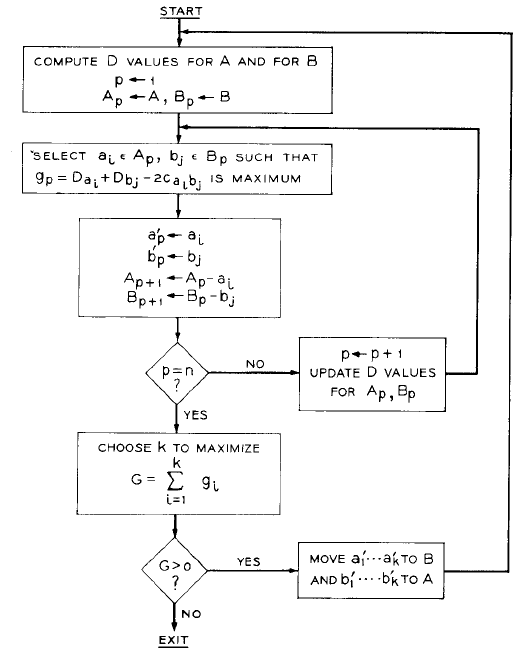
\includegraphics[keepaspectratio,width=0.55\textwidth]{img/03-graphs/kl.png}
                \end{center}
                \caption{A flow diagram of the KL algorithm~\autocite{kl}.} 
                \label{kl-fig}
            \end{figure}
                
            The KL algorithm in its most basic form finds a minimal cut of the graph into two disjoint partitions of the same size. 
            It assumes an undirected graph and is extended to unequally sized partitions and $k$-way partitioning. 
            To decide which node has to be in which partition a cost function $D(v)$ is used. 
            Let $v  \in V_i$ and $i \neq j$. $I(v)$ is called the internal cost of $v$, $E(v)$ is called the external cost of $v$ with
            \[ I(v) = \sum_{u \in V_i} w_{(u, v)} \]
            \[ E(v) = \sum_{s \in V_i} w_{(s, v)} \]
            \[   D(v) = E(v) - I(V)   \]
            The internal cost is thus the sum of all edge weights within a partition incident to a specific vertex, while the external cost is the sum of all edge weights to vertices in the other partition for a specific vertex. 
            The overall cost function is just the difference between external and internal cost.
            The gain of exchanging two vertices between partitions is proven~\autocite{kl} to be --- with $v \in V_i, s \in V_j, i \neq j$
            \[ g = D_v + D_s - 2 w_{(v,s)} \]
            
            The most basic form works as follows.
            \begin{enumerate}
                \item Split the set of vertices into two partitions arbitrarily.
                \item $\forall v \in V$ compute $D(v)$.
                \item Select $v \in V_i, s \in V_j, i \neq j$ such that $g$ is maximal. Exclude them from their partitions.
                \item Update the $D$ values for all remaining nodes in both partitions using 
                \[ u \in V_i \setminus {v}: D'(u) = D(u) + 2 w_{(u, v)} - 2 w_{(u, s)} \]
                \[ x \in V_j \setminus {s}: D'(x) = D(x) + 2 w_{(x, s)} - 2 w_{(s, v)} \]
                \item Go to 3 until the partitions are empty.
                \item choose $k$ to maximize 
                \[ G = \sum^k_{i = 0} g_i \]
                \item If $G > 0$ apply the swaps and go to 2. Else terminate
            \end{enumerate}
            The steps are summarized in the flow diagram in Figure~\ref{kl-fig}.
            Regarding the extensions, an improvement schema is provided to avoid local optima.
            Apply the algorithm to the so created partitions and union the partitions alternatingly (i.e. $A_1 \cup B_2, A_2 \cup B_1$) and use these partitions as initialization of the algorithm.
            In order to create partitions of unequal size with $n_1$ being the minimal desired partition size and $n_2$ the maximal desired partition size, add dummy vertices, such that we have $2n_2$ vertices in total and restrict the number of changes that are allowed to $n_1$.
            For partitioning the graph into $k$-partitions, one needs to split the initial set of vertices into $k$ partitions. 
            Then apply the 2-way partitioning algorithm pairwise to all partitions until convergence.
            
            One pass of the basic form of the algorithm is in $\mathcal{O}(|V|^2 \cdot \log(|V|))$. The $k$-way partitioning algorithm requires per iteration $\binom{k}{2} = \frac{k (k - 1)}{2}$ executions of the algorithm, thus $\mathcal{O}(k^2 \cdot |V|^2 \cdot \log(|V|)$ in total, assuming that the number of iterations is small as shown empirically by the authors~\autocite{kl}. Further improvements were developed in the years after publication, for example a linear time implementation applicable to hypergraphs by Fiduccia and Mattheyses~\autocite{fm}.

        \subsubsection*{Leiden Method}
            The Leiden method~\autocite{traag2019louvain} is an extension of the louvain method.
            It changes and extends the louvain method in three aspects.
            \begin{enumerate}
                \item It changes the quality function introducing an additional resolution parameter.
                \item It incorporates improvements by other authors on how nodes are moved between partitions~\autocite{movd,movc,movb,mova}.
                \item It adds a refinement stage after the contraction of the graph has converged.
            \end{enumerate}
            The quality function that is used by the Leiden method overcomes the problem of the resolution limit~\autocite{traag2011narrow, fortunato2007resolution}.
            It is called the Constant Potts Model~\autocite{potts1952some, traag2011narrow} and defined by 
            \[ CPM = \sum_{u,v \in V}(w_{(u,v)} + \gamma) \delta(u, v) \]
            where $G$ is a graph, $P$ is a partitioning of $G$, $w_{(u,v)}$ is the edge weight between $u$ and $v$, and $\gamma$ is the resolution parameter. 
            Intuitively it controls the coarseness of the partition and replaces the term $\frac{w_u w_v}{2m}$.
            A partition is formed, if its density is at least $\gamma$ and the density between partitions should be less than $\gamma$~\autocite{traag2019louvain}.
            
            \begin{figure}[htp]
                \begin{center}
                    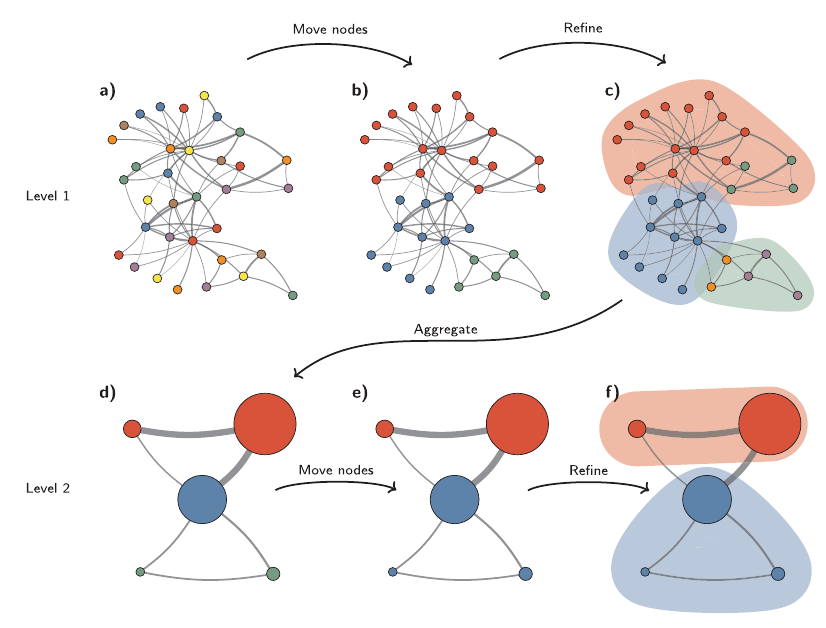
\includegraphics[keepaspectratio,width=0.6\textwidth]{img/03-graphs/leiden.png}
                \end{center}
                \caption{The steps that the leiden algorithm executes~\autocite{traag2019louvain}.} 
                \label{leiden-fig}
            \end{figure}
            
            The node movement is changed in a couple of ways.
            The Leiden algorithm keeps track of which neighbourhoods changed and only visits these nodes again, in contrast to louvain which keeps iterating all nodes\autocite{movb, movc}.
            Initially it adds all nodes to a queue, removes the first on and adds the nodes neighbourhood to the queue only if it was moved.
            
            The refinement stage is added after moving nodes between communities and before aggregating the communities into a new graph.
            Starting with the partitioning $P$, the algorithm derives a refined partitioning $P_{\text{ref}}$.
            First all nodes are again initialized as an own singleton community. 
            Now nodes which are in their own community $C^i_{\text{ref}}$ can again be merged with into another community $C^j_{\text{ref}}$, but this time only with those from the same community in the previous partitioning $C \in P$. 
            In essence it forms from a given partitioning a finer grained partitioning within the communities.
            Additionally not the merge with the highest increase in the quality function is chosen but the choice is made randomly with higher probability for better quality values, in order to avoid getting stuck in local optima~\autocite{mova}.
            
            Empirically, the Leiden algorithm converges faster with a higher modularity score, whith appropriate values for $\gamma$. A good value to start is $\gamma = \frac{1}{2}$, which results in an approximation of the louvain algorithm's quality function --- the modularity of Newman and Girvan~\autocite{girvan2002community}.
                
\section{Database Architecture}\label{db-arch}
    The reason why we use databases is twofold:
    First, every computer is equipped with different kinds of memory, which differ in size, capacity, speed and price per byte. 
    This induces the so called memory hierarchy, the principle, that few fast, expensive, low capacity memory is used close to the central processing unit, that gets layerwise augmented with inccreasingly slower, less expensive, higher capacity memory. 
    The last layer, which has the highest capacity, defines the overall capacity, while the smallest one is a crucial factor for performance.
    Thus what is shown as secondary storage in Figure~\ref{mem-hier} is orders of magnitude slower in terms of both latency and throughput.
    But it is also able to store orders of magnitude more data. 
    \begin{figure}[htp]
        \begin{center}
        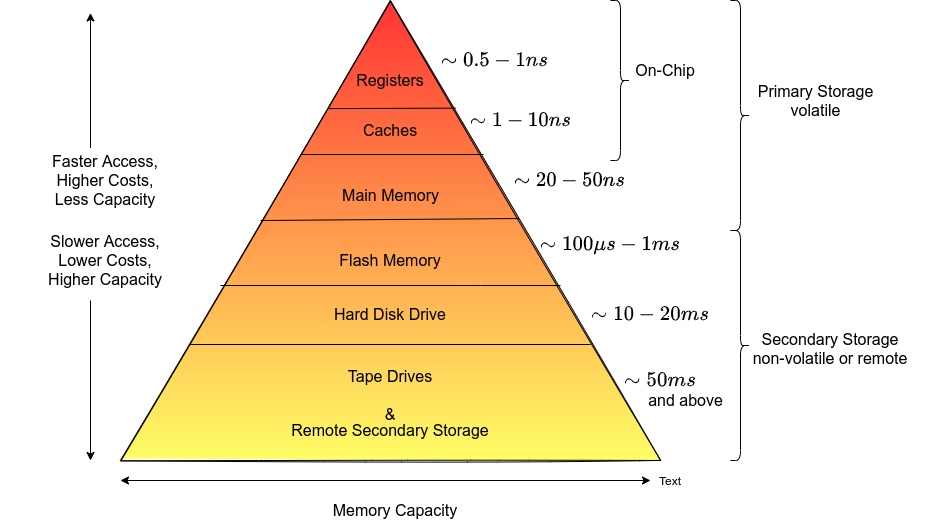
\includegraphics[keepaspectratio,width=0.8\textwidth]{img/04-databases/mem-hierarch.png}
        \end{center}
        \caption{The memory hierarchy used in today's computing systems.} 
        \label{mem-hier}
    \end{figure}
    In order to mitigate the effects of this, the accesses between primary and secondary memory need to be handled very carefully for data intensive --- also called IO bound --- applications.
    Second, the operating system (OS) actually handles the first reason. 
    However application specific payloads enable further optimizations when it comes to how data is stored and accessed.
    Put differently, the operating system is not able to infer certain information, as it does not constrain how data is stored, and as it does not profile in what patterns data is referenced or queried.
    Databases take care of these issues by different mechanisms, which will be lined out from a high level perspective, in order to understand how a database works on its architectural lower levels.
    Put differently, we are not going to discuss query processing, transactions, concurrency related components and recovery facilities.
    Most of the information below is outlined comprehensively in~\autocite{ramakrishnan2000database, silberschatz1997database}
    
    Let us consider the high level architecture of a general database management systems as shown in Figure~\ref{dbms_arch} --- with a focus on the storage and access elements.

    \begin{figure}[htp]
    \begin{center}
    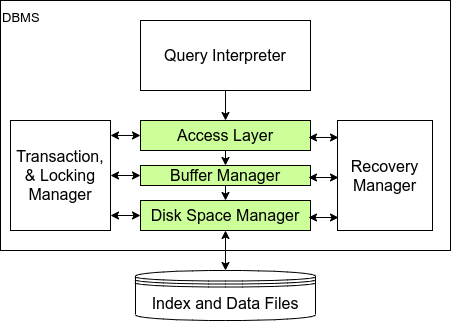
\includegraphics[keepaspectratio,width=.5\textwidth]{img/04-databases/RDBMS.png}
    \end{center}
    \caption{The typical structure of a relational database management system~\autocite{ramakrishnan2000database}.}
    \label{dbms_arch}
    \end{figure}

    The disk space manager, sometimes also called storage manager, handles de-/allocations, reads \& writes and provides the concept of a block: One or many physical disk blocks are grouped to a logical disk block.
    These logical disk blocks are again grouped and brought into main memory (RAM) --- these groups are called a page.
    Optimally both a disk block and a page are of the same size or at least a multiple of each other. 
    Further the database needs to keep track of free blocks in the file: 
    A linked list or a directory must record free blocks and some structure needs to keep track of the free slots either globally or per block. 
    Data locality is a concept that we examine closely in an extra chapter later on.
    To summarize the two most important objectives of a storage manager are to
    \begin{enumerate} 
     \item take care of (de-)allocations of disk space,
     \item abstract storing data on a physical device using the operating system: Files, split into logical disk blocks, accessed using OS facilities, and
     \item provide data structures in order to maintain records within a file, blocks.
    \end{enumerate}
    
    A buffer manager is used to mediate between external storage and main memory. 
    It provides the concept of a page and maintains a designated pre-allocated area of main memory --- called the buffer pool --- to load, cache and evict pages into or from main memory~\autocite{ramakrishnan2000database}.
    A conceptual illustration of this is shown in \ref{buf-man}.
    It's objective is to minimize the number of disk reads to be executed by caching, pre-fetching and the usage of suitable replacement policies. 
    It also needs to take care of allocating a certain fraction of pages to each transaction.

    \begin{figure}[htp]\label{dbms_memory}
        \begin{center}
        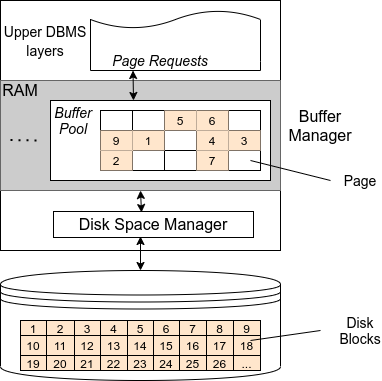
\includegraphics[keepaspectratio,height=0.4\textheight,width=0.5\textwidth]{img/04-databases/RDBMS_memory_view.png}
        \end{center}
        \caption{A visualization of the interaction of a database with memory~\autocite{ramakrishnan2000database}.}
        \label{buf-man}
    \end{figure}

    The final component that is crucial to the storage of data the  of a database management system is the file and record layout, along with possible index structures --- also called the access layer. 
    In order to store data a DBMS may either use one single or multiple files to maintain records. 

    A file consists of a set of blocks split into slots.
    A slot stores one record with each record containing a set of fields.
    Records can be layout in row or column major order.
    That is one can store sequences of tuples or sequences of fields.
    The former is beneficial if a lot of update, insert or delete operations are committed to the database, while the latter optimizes the performance when scans and aggregations are the most typical queries to the system.
    Records may be of fixed or of variable size, depending on the types of their fields. 
    Another option is to store the structure of the records along with pointers to the values of their fields in one files and the actual values in one or multiple separate files. 
    Also distinct types of tables can be stored in different files. 
    For example entities and relations can be stored in different files with references to each other, thus enabling the layout of these two to be specialized to their structure and usage in queries.

    Files may either organize their records in random order (heap file), sorted or using a hash function on one or more fields. 
    All of these approaches have upsides and downsides when it comes to scans, searches, insertions, deletions and updates. 

    To mitigate the effect that result from selecting one file organization or another, one record organization or another, the concept of an index has been introduced. 
    Indexes are auxiliary structures to speed up certain operations or queries that depend on one field. 
    Indexes may be clustered or unclustered. 
    An index over field $F$ is called clustered if the underlying data file is sorted according to the values of $F$. 
    Otherwise the index is called unclustered
    In a similar way indexes can be sparse or dense. 
    A sparse index has less index entries than records, mostly one index entry per block. 
    This can of course only be done for clustered indexes as the sorting of the data file keeps the elements between index keys in order. 
    An index is dense if there is a one to one correspondence between records and index entries. 
    All unclustered indexes are dense indexes.
    There are different variants of storing index entries which have again certain implications on the compactness of the index and the underlying design decisions.
    Finally, there are operators that act upon and use the above structures and mechanisms. 
    Logical operators define an algebraic operation used to process a query.
    Physical operators implement the operation described by logical operators. For each logical operator there may exist multiple different physical implementations using different access methods.

    All these considerations make choosing different file splits, layouts, orderings, addressing schemes, management structures, de-/allocation schemes and indexes a complex set of dependent choices. 
    These depend mainly on the structure of the data to be stored and the queries to be run.

\section{Static Locality-optimizing Layout Methods}
    \subsection*{Bondhu: An alternating Ordering Scheme}
    Bondhu~\autocite{hoque2012disk} is a data layout technique for online social network data. 
    The authors define the cost of a placement similar to the ranking locality above, with $r$ defined as before: \[ \text{cost} = \sum_{(u, v) \in E} |r(v) - r(u)| \]   
    Without citing G-Store, Hoque and Gupta propose to use the multilevel partitioning algorithm implemented in METIS~\autocite{karypis} to partition the graph. Additionally the authors propose to use the Louvain method~\autocite{blondel2008fast} to find communities, but they don't provide results on this method. The louvain method is described in more detail in the next section. \\
    
    \begin{figure}[htp]
        \begin{center}
            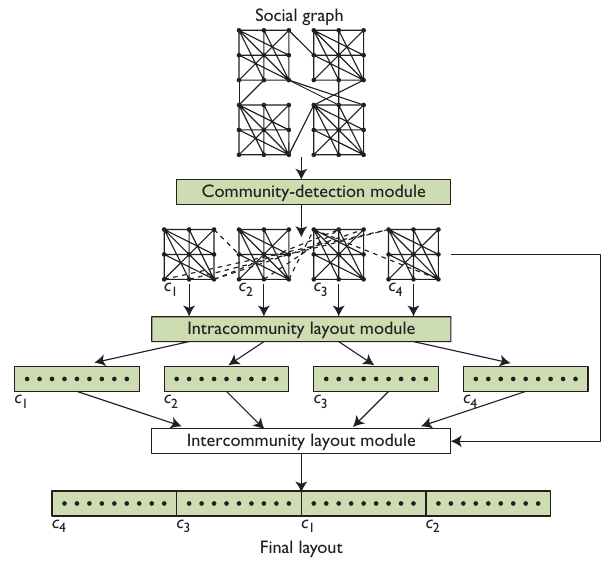
\includegraphics[keepaspectratio,width=0.8\textwidth]{img/06-rel_w/bondhu.png}
        \end{center}
        \caption{Broad steps performed by the bondhu algorithm~\autocite{hoque2012disk}.} 
        \label{bondhu-fig}
    \end{figure}

    The authors propose an incremental placement schema within a block:
    Place the node with the highest degree in the middle of the block, then select the node with the heaviest edge connected to the first node and place it next to the first node. 
    After these two placements, a new graph is created, where the two already placed nodes are merged and their relationships are aggregated. 
    The node with the next heaviest edge is selected and placed alternatingly. The previous two steps are repeated until all nodes are placed within blocks.
    This is done for every community.
    In the final part of the method, the intercommunity layout is derived. 
    Here each community is a vertex and the edges between those are just the accumulated edges of the underlying graph. 
    After creating the graph the previous alternating placement schema is applied.
    
    \subsection*{Louvain-like Formation and RCM-based Ordering}
        As a first step, contration algorithm that optimizes the modularity or the CPM~\autocite{traag2011narrow, potts1952some} function is executed.
        During the contraction step of the louvain or the leiden algorithm~\autocite{traag2019louvain}, it is easy to stop merging when communities reach a certain number if nodes.
        That is as soon as a community has $\frac{\text{Block Size}}{\text{node size}}$ nodes, then don't consider merging nodes into it anymore.
        This results in block sized partitions.
        The aggregation step of these algorithms can then be performed as is. 
        Afterwards executing the algorithm in its standard form yields a hierarchy of graphs, similar to the method employed in G-Store.
    
        This can then be used to achieve an ordering of the blocks:
        Uncoarsen the graph by applying the Dewey numbering scheme~\autocite{dewey1894decimal}, employed by ICBL and G-Store.
        Additionally, an heuristic for improving the vertex ordering can be applied layerwise. 
        A recent comprehensive survey of minimum linear arrangement approximation algorithms can be found in~\autocite{barik2020vertex}.
        An appealing option would be to apply the reverse Cuthill-McKee (RCM) algorithm~\autocite{Cuthill1969ReducingTB}, that approximates the solution in $\mathcal{O}(|V| \cdot \text{deg}{V}) = \mathcal{O}(|E|)$. 
        It first finds a peripheral vertex.
        Then it starts a modified version of the breadth first search, that sorts the nodes by traversal order and degree.
        The quality of the algorithm is highly dependent on the input graph.
        As the input graph is the already approximately ordered graph from the last level, the effects of input ordering should be mitigated.
        Results for the algorithm compared to other state of the art methods are described by Barik et al.~\autocite{barik2020vertex}.
        
        After the algorithms above are finished, the vertices are layed out in this order to file. 
        The relationships are written to file in the very same order by grouping and storing the outgoing edges of a vertex together and following the vertex order.
        That is, the outgoing edges of the vertex stored at the first slot in the vertex file are stored beginning at the first slot of the edge file. 
        The outgoing edges of the second node start right after the edge group of the first node and so on.
        This scheme is motivated by the asusmption that traversals in directed graphs follow the edge direction.

\chapter{Evaluation Data}
\begin{table}
	\begin{center}
		 \begin{tabular}[c]{c c c c c c} \toprule
			  & BFS & DFS & Dijkstra & $A^*$  & ALT \\ \midrule 
 			\multirow{2}{*}{Natural}  & 118 & 112 & 113 & 16 & 8 \\ 
 				 & 1025 & 1026 & 1026 & 158 & 67 \\ 
 				&&&&& \\[-0.5em]
 			\multirow{2}{*}{Random}  & 120 & 121 & 118 & 81 & 102 \\ 
 				 & 1036 & 1028 & 1035 & 772 & 940 \\ 
 				&&&&& \\[-0.5em]
 			\multirow{2}{*}{Louvain}  & 74 & 66 & 79 & 10 & 15 \\ 
 				 & 749 & 714 & 647 & 101 & 196 \\ 
 				&&&&& \\[-0.5em]
 			\multirow{2}{*}{G-Store}  & 75 & 89 & 75 & 13 & 24 \\ 
 				 & 581 & 652 & 570 & 149 & 366 \\ 
 				&&&&& \\[-0.5em]
 			\multirow{2}{*}{ICBL}  & 96 & 86 & 66 & 12 & 40 \\ 
 				 & 695 & 734 & 819 & 107 & 349 \\ 
 				&&&&& \\[-0.5em]
 					\end{tabular}  
  	 \end{center}
	 \caption{Comparison of IOs per method, query and record type on the C. elegans dataset with unsorted incidence lists.}
	 \label{ce-uns}
\end{table}

\begin{table}
	\begin{center}
		 \begin{tabular}[c]{c c c c c c} \toprule
			  & BFS & DFS & Dijkstra & $A^*$  & ALT \\ \midrule 
 			\multirow{2}{*}{Natural}  & 114 & 114 & 111 & 11 & 35 \\ 
 				 & 952 & 944 & 952 & 110 & 366 \\ 
 				&&&&& \\[-0.5em]
 			\multirow{2}{*}{Random}  & 122 & 114 & 121 & 71 & 97 \\ 
 				 & 961 & 960 & 957 & 665 & 785 \\ 
 				&&&&& \\[-0.5em]
 			\multirow{2}{*}{Louvain}  & 83 & 82 & 69 & 14 & 17 \\ 
 				 & 222 & 389 & 145 & 60 & 99 \\ 
 				&&&&& \\[-0.5em]
 			\multirow{2}{*}{G-Store}  & 73 & 86 & 75 & 16 & 30 \\ 
 				 & 178 & 280 & 228 & 77 & 168 \\ 
 				&&&&& \\[-0.5em]
 			\multirow{2}{*}{ICBL}  & 84 & 81 & 67 & 12 & 46 \\ 
 				 & 146 & 167 & 355 & 106 & 197 \\ 
 				&&&&& \\[-0.5em]
 					\end{tabular}  
  	 \end{center}
	 \caption{Comparison of IOs per method, query and record type on the C. elegans dataset with sorted incidence lists.}
	 \label{ce-s}
\end{table}


\begin{table}
	\begin{center}
		 \begin{tabular}[c]{c c c c c c} \toprule
			  & BFS & DFS & Dijkstra & $A^*$  & ALT \\ \midrule 
 			\multirow{2}{*}{Natural}  & 970 & 972 & 972 & 326 & 774 \\ 
 				 & 39123 & 39114 & 39123 & 22834 & 34759 \\ 
 				&&&&& \\[-0.5em]
 			\multirow{2}{*}{Random}  & 973 & 966 & 971 & 99 & 132 \\ 
 				 & 39105 & 39097 & 39106 & 8389 & 10319 \\ 
 				&&&&& \\[-0.5em]
 			\multirow{2}{*}{Louvain}  & 605 & 638 & 773 & 321 & 400 \\ 
 				 & 27778 & 29728 & 30127 & 28255 & 24875 \\ 
 				&&&&& \\[-0.5em]
 			\multirow{2}{*}{G-Store}  & 685 & 647 & 751 & 206 & 331 \\ 
 				 & 24234 & 28923 & 25016 & 10397 & 14441 \\ 
 				&&&&& \\[-0.5em]
 			\multirow{2}{*}{ICBL}  & 771 & 633 & 585 & 347 & 162 \\ 
 				 & 30453 & 21861 & 25379 & 21617 & 10448 \\ 
 				&&&&& \\[-0.5em]
 					\end{tabular}  
  	 \end{center}
	 \caption{Comparison of IOs per method, query and record type on the email dataset with unsorted incidence lists.}
	 \label{email-uns}
\end{table}

\begin{table}
	\begin{center}
		 \begin{tabular}[c]{c c c c c c} \toprule
			  & BFS & DFS & Dijkstra & $A^*$  & ALT \\ \midrule 
 			\multirow{2}{*}{Natural}  & 952 & 947 & 966 & 316 & 762 \\ 
 				 & 29223 & 29221 & 29225 & 16340 & 25755 \\ 
 				&&&&& \\[-0.5em]
 			\multirow{2}{*}{Random}  & 908 & 949 & 932 & 43 & 72 \\ 
 				 & 29236 & 29231 & 29237 & 4127 & 5432 \\ 
 				&&&&& \\[-0.5em]
 			\multirow{2}{*}{Louvain}  & 629 & 592 & 539 & 407 & 399 \\ 
 				 & 5169 & 8945 & 8247 & 8042 & 4978 \\ 
 				&&&&& \\[-0.5em]
 			\multirow{2}{*}{G-Store}  & 748 & 650 & 549 & 204 & 111 \\ 
 				 & 8024 & 6454 & 6490 & 4488 & 1010 \\ 
 				&&&&& \\[-0.5em]
 			\multirow{2}{*}{ICBL}  & 558 & 733 & 664 & 164 & 268 \\ 
 				 & 4504 & 9007 & 4849 & 6316 & 5776 \\ 
 				&&&&& \\[-0.5em]
 					\end{tabular}  
  	 \end{center}
	 \caption{Comparison of block IOs per method, query and record type on the email dataset with sorted incidence lists.}
	 \label{email-s}
\end{table}


\begin{table}
	\begin{center}
		 \begin{tabular}[c]{c c c c c c} \toprule
			  & BFS & DFS & Dijkstra & $A^*$  & ALT \\ \midrule 
 			\multirow{2}{*}{Natural}  & 317072 & 317071 & 317071 & 88454 & 239225 \\ 
 				 & 1338193 & 1314632 & 1344250 & 598168 & 1135678 \\ 
 				&&&&& \\[-0.5em]
 			\multirow{2}{*}{Random}  & 317063 & 317064 & 317070 & 2338 & 91026 \\ 
 				 & 1338218 & 1314495 & 1344206 & 20784 & 506800 \\ 
 				&&&&& \\[-0.5em]
 			\multirow{2}{*}{Louvain}  & 209269 & 231464 & 190242 & 27762 & 219532 \\ 
 				 & 1003659 & 906895 & 846871 & 249979 & 723742 \\ 
 				&&&&& \\[-0.5em]
 			\multirow{2}{*}{G-Store}  & 250482 & 187065 & 215604 & 16340 & 97658 \\ 
 				 & 842998 & 972704 & 752748 & 156619 & 409640 \\ 
 				&&&&& \\[-0.5em]
 					\end{tabular}  
  	 \end{center}
	 \caption{Comparison of IOs per method, query and record type on the DBLP dataset with unsorted incidence lists.}
	 \label{dblp-uns}
\end{table}

\begin{table}
	\begin{center}
		 \begin{tabular}[c]{c c c c c c} \toprule
			  & BFS & DFS & Dijkstra & $A^*$  & ALT \\ \midrule 
 			\multirow{2}{*}{Natural}  & 317072 & 317064 & 317076 & 15934 & 242959 \\ 
 				 & 1335990 & 1322882 & 1341846 & 145842 & 1141861 \\ 
 				&&&&& \\[-0.5em]
 			\multirow{2}{*}{Random}  & 317058 & 317065 & 317062 & 2725 & 88404 \\ 
 				 & 1335872 & 1322426 & 1341851 & 23601 & 487566 \\ 
 				&&&&& \\[-0.5em]
 			\multirow{2}{*}{Louvain}  & 190245 & 218779 & 206096 & 32042 & 174006 \\ 
 				 & 495939 & 300461 & 179801 & 65190 & 426641 \\ 
 				&&&&& \\[-0.5em]
 			\multirow{2}{*}{G-Store}  & 187067 & 221947 & 231457 & 19841 & 127806 \\ 
 				 & 486164 & 285141 & 287917 & 87398 & 168100 \\ 
 				&&&&& \\[-0.5em]
 					\end{tabular}  
  	 \end{center}
	 \caption{Comparison of IOs per method, query and record type on the DBLP dataset with sorted incidence lists.}
	 \label{dblp-s}
\end{table}


\begin{table}
	\begin{center}
		 \begin{tabular}[c]{c c c c c c} \toprule
			  & BFS & DFS & Dijkstra & $A^*$  & ALT \\ \midrule 
 			\multirow{2}{*}{Natural}  & 334854 & 334846 & 334854 & 23591 & 206718 \\ 
 				 & 1275141 & 1261562 & 1278263 & 121074 & 859489 \\ 
 				&&&&& \\[-0.5em]
 			\multirow{2}{*}{Random}  & 334844 & 334839 & 334845 & 4630 & 81595 \\ 
 				 & 1274993 & 1261169 & 1278126 & 21735 & 340428 \\ 
 				&&&&& \\[-0.5em]
 			\multirow{2}{*}{Louvain}  & 254490 & 237746 & 267880 & 7217 & 90032 \\ 
 				 & 994592 & 971234 & 1022546 & 33642 & 363483 \\ 
 				&&&&& \\[-0.5em]
 			\multirow{2}{*}{G-Store}  & 217652 & 254487 & 237742 & 17030 & 169893 \\ 
 				 & 969107 & 946004 & 945848 & 88412 & 856992 \\ 
 				&&&&& \\[-0.5em]
 					\end{tabular}  
  	 \end{center}
	 \caption{Comparison of IOs per method, query and record type on the Amazon dataset with unsorted incidence lists.}
	 \label{amazon-uns}
\end{table}

\begin{table}
	\begin{center}
		 \begin{tabular}[c]{c c c c c c} \toprule
			  & BFS & DFS & Dijkstra & $A^*$  & ALT \\ \midrule 
 			\multirow{2}{*}{Natural}  & 334831 & 334831 & 334838 & 29305 & 213728 \\ 
 				 & 1271978 & 1253135 & 1275516 & 148144 & 881883 \\ 
 				&&&&& \\[-0.5em]
 			\multirow{2}{*}{Random}  & 334826 & 334833 & 334829 & 5267 & 105294 \\ 
 				 & 1271472 & 1253034 & 1275273 & 24768 & 446134 \\ 
 				&&&&& \\[-0.5em]
 			\multirow{2}{*}{Louvain}  & 210935 & 194200 & 237722 & 7544 & 105341 \\ 
 				 & 531443 & 184171 & 327139 & 16324 & 97106 \\ 
 				&&&&& \\[-0.5em]
 			\multirow{2}{*}{G-Store}  & 224334 & 254463 & 210939 & 20196 & 186835 \\ 
 				 & 349005 & 395952 & 192827 & 47784 & 418902 \\ 
 				&&&&& \\[-0.5em]
 					\end{tabular}  
  	 \end{center}
	 \caption{Comparison of IOs per method, query and record type on the amazon dataset with sorted incidence lists.}
	 \label{amazon-s}
\end{table}


\begin{table}
	\begin{center}
		 \begin{tabular}[c]{c c c c c c} \toprule
			  & BFS & DFS & Dijkstra & $A^*$  & ALT \\ \midrule 
 			\multirow{2}{*}{Natural}  & 1134885 & 1134874 & 1134887 & 520744 & 626139 \\ 
 				 & 3376451 & 3180208 & 3434910 & 3029489 & 2837347 \\ 
 				&&&&& \\[-0.5em]
 			\multirow{2}{*}{Random}  & 1134878 & 1134879 & 1134885 & 494930 & 900538 \\ 
 				 & 3378223 & 3180625 & 3436253 & 2995538 & 3134437 \\ 
 				&&&&& \\[-0.5em]
 			\multirow{2}{*}{Louvain}  & 624186 & 805764 & 714975 & 130763 & 464393 \\ 
 				 & 2432604 & 2385390 & 2748602 & 1315246 & 1918687 \\ 
 				&&&&& \\[-0.5em]
 			\multirow{2}{*}{G-Store}  & 817115 & 783068 & 749022 & 24225 & 128005 \\ 
 				 & 2431757 & 1780594 & 2679796 & 326708 & 957401 \\ 
 				&&&&& \\[-0.5em]
 					\end{tabular}  
  	 \end{center}
	 \caption{Comparison of IOs per method, query and record type on the C. elegans dataset with unsorted incidence lists.}
	 \label{yt-uns}
\end{table}

\begin{table}
	\begin{center}
		 \begin{tabular}[c]{c c c c c c} \toprule
			  & BFS & DFS & Dijkstra & $A^*$  & ALT \\ \midrule 
 			\multirow{2}{*}{Natural}  & 1134879 & 1134869 & 1134870 & 466807 & 673661 \\ 
 				 & 3369934 & 3274601 & 3427327 & 2760899 & 2877905 \\ 
 				&&&&& \\[-0.5em]
 			\multirow{2}{*}{Random}  & 1134841 & 1134858 & 1134858 & 545467 & 743401 \\ 
 				 & 3372967 & 3274050 & 3428718 & 3193624 & 2932793 \\ 
 				&&&&& \\[-0.5em]
 			\multirow{2}{*}{Louvain}  & 885148 & 760368 & 828413 & 129288 & 439661 \\ 
 				 & 1238579 & 1003650 & 809341 & 308880 & 733981 \\ 
 				&&&&& \\[-0.5em]
 			\multirow{2}{*}{G-Store}  & 771704 & 907899 & 646850 & 21961 & 112100 \\ 
 				 & 550333 & 1055840 & 958365 & 147532 & 326985 \\ 
 				&&&&& \\[-0.5em]
 					\end{tabular}  
  	 \end{center}
	 \caption{Comparison of IOs per method, query and record type on the YouTube dataset with sorted incidence lists.}
	 \label{yt-s}
\end{table}



\end{document}
